\documentclass[titlepage,a4paper]{article}

\usepackage{a4wide}
\usepackage[colorlinks=true,linkcolor=black,urlcolor=blue,bookmarksopen=true]{hyperref}
\usepackage{bookmark}
\usepackage{fancyhdr}
\usepackage[spanish]{babel}
\usepackage[utf8]{inputenc}
\usepackage[T1]{fontenc}
\usepackage{graphicx}
\usepackage{float}
\usepackage{tabularx}
\usepackage{tabto}
\usepackage{pgfgantt}
\usepackage{xcolor}
\usepackage{wrapfig}
\usepackage[utf8]{inputenc}
\usepackage{graphicx}
\usepackage{subcaption}
\usepackage{hyperref}




\pagestyle{fancy} % Encabezado y pie de página
\fancyhf{}
\fancyhead[L]{El Cuarteto Imperial - TP1}
\fancyhead[R]{75.06 Organización de Datos - FIUBA}
\renewcommand{\headrulewidth}{0.4pt}
\fancyfoot[C]{\thepage}
%\renewcommand{\footrulewidth}{0.4pt}
\renewcommand{\baselinestretch}{1,5}

\begin{document}
\begin{titlepage} % Carátula
    
	\hfill
\includegraphics[width=6cm]{logofiuba.jpg}
    \centering
    \vskip1cm
    \Huge \textbf{UBA - Facultad de Ingeniería}
    \vskip0.25cm
    \LARGE{Departamento de Computación}    
    \vskip0.25cm
    \LARGE{Organización de Datos (75.06)}
    \vskip1.2cm
    \vskip0.3cm
    \Huge \textbf{Trabajo Práctico 1} 
    \vskip0.5cm
    \LARGE{1er cuatrimestre - 2020}
    \vskip1.5cm
    \large
  	\begin{center}
    \begin{tabular}{||{7cm}||{2cm}||{6cm}||}
     \hline
     \multicolumn{3}{||c||}{GRUPO: \textbf{El Cuarteto Imperial}} \\ [0.5ex]
     \hline
     \hline
     \centering{\textbf{Alumno}} & \textbf{Padrón} & \textbf{Mail}\\ \hline
          LARREA BUENDÍA, Hugo Marcelo & 102140 & hlarrea@fi.uba.ar\\ \hline
          MARTINEZ SASTRE, Gonzalo Gabriel & 102321 & \normalsize gonzalomartinezsastre@gmail.com \\ \hline
          RIEDEL, Nicolás Agustín & 102130 & nriedel@fi.uba.ar\\ \hline
          ZBOGAR, Ezequiel & 102216 & ezbogar@fi.uba.ar\\ \hline
    \end{tabular}
    \end{center}
     
    \end{titlepage}
    
\tableofcontents
\newpage
\setlength{\parskip}{2mm}

\section{Resumen}
En el presente Trabajo Práctico se lleva a cabo un análisis exploratorio en base a un conjunto de datos compuesto por \textit{Tweets} de diferentes partes del mundo. Como particularidad gran parte de estos \textit{Tweets} tienen palabras que pertenecen a la terminología utilizada para referirse a accidentes o catástrofes.

El objeto de dicho análisis es organizar la información que aportan los datos de manera que sea plausible detectar patrones de comportamiento, tendencias, valores atípicos (también llamados \textit{outliers}), resultados inesperados, saltos o discontinuidades, concentraciones de valores, formas de distribución, o cualquier otro tipo de característica destacable, de manera tal que permitan posteriormente elaborar conclusiones sobre los mismos.

A lo largo de este trabajo se analizan diversos componentes de los \textit{Tweets}. Siendo estos elementos el texto que contienen, la ubicación desde donde fue hecho el \textit{Tweet}, la \textit{Keyword} asociada y si efectivamente el \textit{Tweet} habla sobre un desastre o no.

En el análisis del texto de los \textit{Tweets} se estudia la longitud de los mismos (tanto en términos de caracteres como en palabras), las palabras que más aparecen en estos, las palabras que aparecen mucho más en \textit{Tweets} que hablan sobre un desastre, las palabras que no suelen aparecer en los \textit{Tweets} sobre desastres, y si existe una relación entre si este habla sobre una tragedia y los caracteres especiales que contiene.

En el análisis por \textit{Keywords} se estudio la relación entre el \textit{Keyword} asociado al \textit{Tweet} y su longitud, tanto en caracteres como en palabras. También se busco una conexión entre la \textit{Keyword} y el \textit{Target} del \textit{Tweet}. Por último se examinó cuales son las \textit{Keywords} con más apariciones en el set de datos.

En el análisis por ubicación se estudió qué cantidad de \textit{Tweets} tienen efectivamente una localización valida; dentro del grupo que efectivamente la tiene se procede a buscar cual es la ubicación con mayor cantidad de \textit{Tweets}, con mayor porcentaje de \textit{Tweets} que hablan sobre un desastre y luego se realiza un análisis de los sitios de mayor interés.




\newpage

\section{Introducción}\label{sec:intro}

    \textit{Twitter} se ha convertido en un importante canal de comunicación en los últimos años. El mundo globalizado en el que vivimos y el uso cada vez mayor de dispositivos como  \textit{smartphones} y computadoras permiten una comunicación veloz entre personas que se encuentren en distintas partes del mundo. Uno de los usos más relevantes que se le puede dar a esta nueva forma de comunicación es la de informar cualquier tipo de emergencia que estén observando en tiempo real, pero no siempre se utilizan con ese fin y muchas veces es difícil diferenciar cuando una persona esta efectivamente haciendo referencia a un desastre/accidente y cuando no.

    El objetivo de este informe es exponer los resultados del análisis exploratorio realizado en base al set de datos provisto por la cátedra. El mismo consiste en un conjunto de \textit{Tweets} que pueden estar relacionados con desastres/accidentes (ya sean de origen natural o provocado por el ser humano) o no.
    
    La finalidad de este informe es mediante un análisis del set de datos, encontrar patrones entre los \textit{Tweets} y, en base a ello, llegar a conclusiones que nos ayuden a identificar más fácilmente cuando un \textit{Tweet} hace referencia a desgracia o no. 
    
    La información provista por el conjunto de datos para cada \textit{Tweet} se describe a continuación:

    \begin{itemize}
        \item \textbf{\textit{Id}}: Identificador único de cada \textit{Tweet}.
        \item \textbf{\textit{Texto}}: Texto del \textit{Tweet}.
        \item \textbf{\textit{Locación}}: El lugar de procedencia del \textit{Tweet}. 
        \item \textbf{\textit{Keyword}}: Una palabra particular relacionada al \textit{Tweet}.
        \item \textbf{\textit{Target}}: Representa si el \textit{Tweet} habla acerca de un desastre (1) o no (0)
    \end{itemize}
 
    En base a esto, se busca encontrar cualquier tipo de patrón o relación entre los distintos campos y características de los \textit{Tweets} (salvo el \textit{Id} debido a que éste es diferente para cada \textit{Tweet} y no presenta información de interés).
    
    El lenguaje de programación utilizado fue \textit{Python}. Adicionalmente, se utilizaron las siguientes herramientas: \textit{Git} y \textit{Github} como programas de control de versiones, \textit{Jupyter} como entorno de desarrollo y las siguientes bibliotecas: \textit{Pandas}, \textit{Numpy}, \textit{Mathplotlib}, \textit{Bokeh}, \textit{PIL}, \textit{Wordcloud}, \textit{Math}, \textit{Seaborn} y \textit{Geopandas}.
    
    Cabe destacar que a lo largo de todo este trabajo se tomó como convención llamar como verdaderos o veraces a aquellos \textit{Tweets} que realmente tratan sobre un desastre, y como falsos o no veraces a aquellos que no lo hacen.
    
    \newpage
    \section{Análisis del texto de los \textit{Tweets}}\label{sec:intro}
    
    Se comienza el análisis del conjunto de datos con un estudio del contenido de los \textit{Tweets}. Para ello, como paso inicial se busca observar rasgos superficiales de los mismos, tales como la extensión de su texto tanto en palabras como en caracteres.
    
    \begin{figure}[H]
    \centering
    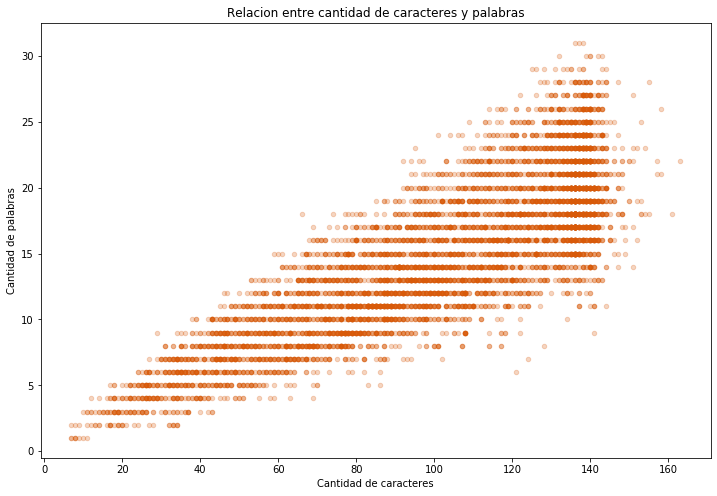
\includegraphics[width=1\textwidth]{graficos/Analisis Lexico Grafico/relacion_entre_cantidad_caracteres_palabras.png}
    \caption{}  
    \end{figure}
    
    En esta visualización cada punto representa un \textit{Tweet} de los 7613 que conforman el set de datos. Como se puede observar, no se muestra ningún resultado inesperado puesto que es entendible que los \textit{Tweets} con mayor cantidad de palabras tiendan a estar compuestos por un mayor número de caracteres.
    
     \subsection{Análisis de las palabras más usadas}
    
    A continuación, se procede a realizar un estudio en profundidad del contenido de los mismos, primero buscando las palabras más repetidas (sin distinguir entre mayúsculas y minúsculas) con el objetivo de detectar temáticas predominantes. El resultado obtenido es el siguiente:
    
    \begin{figure}[H]
    \centering
    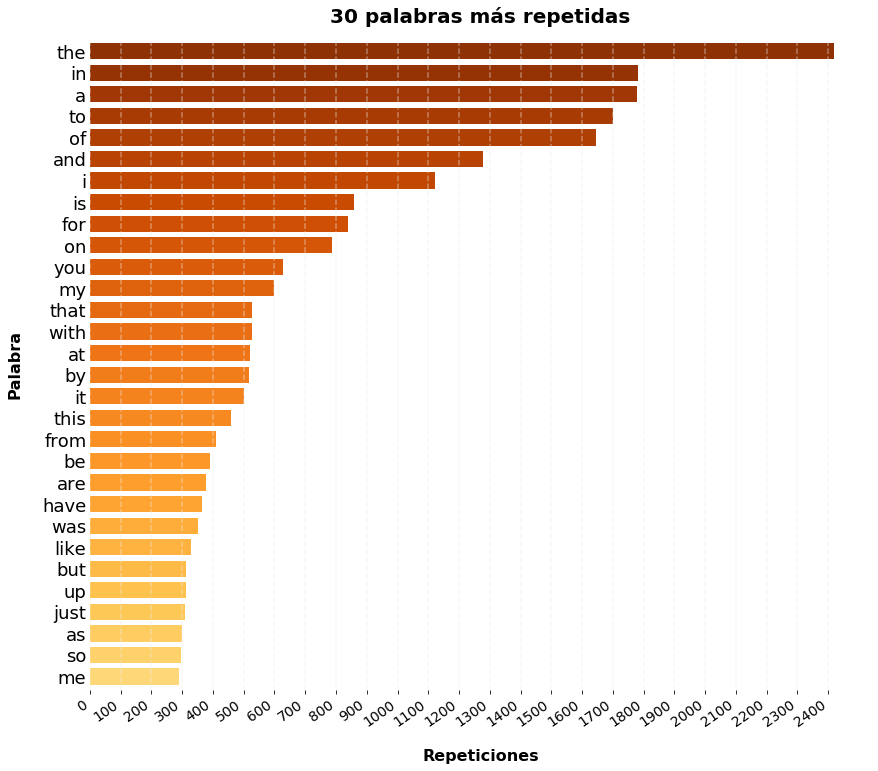
\includegraphics[width=1\textwidth]{graficos/Analisis Lexico Grafico/top30MasUsadas.png}
    \caption{}  
    \end{figure}
    
    
    Este resultado es el esperado, debido a que en el idioma inglés (el predominante en el set de datos) las palabras más usadas son preposiciones, pronombres personales y artículos.
    
    Se procede a filtrar tanto los artículos como las preposiciones  con el fin de apreciar qué palabras (además de ellas) son repetidas a menudo. El resultado fue el siguiente:

    \begin{figure}[H]
    \centering
    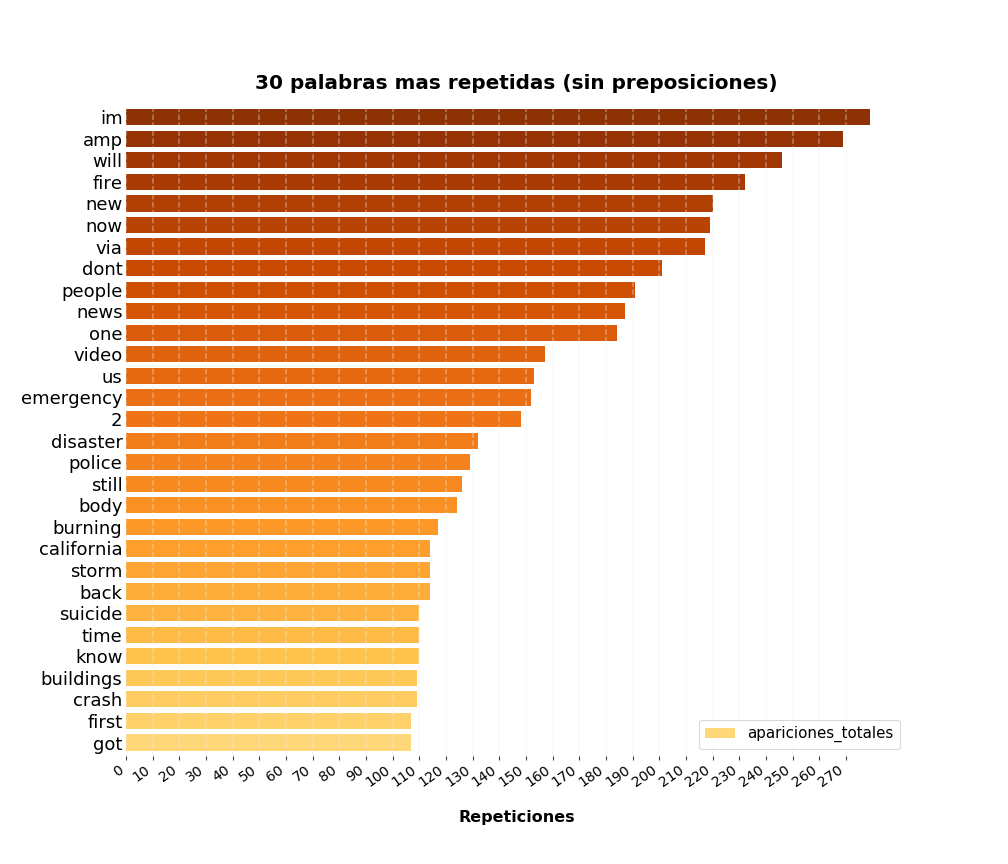
\includegraphics[width=1\textwidth]{graficos/Analisis Lexico Grafico/30masRepetidasFiltrado.png}
    \caption{}  
    \end{figure}
    
    Esto también esperable, ya que la mayoría de las palabras están relacionadas a desastres o a la comunicación de los mismos, lo cual se entiende ya que es el contenido del set de datos.

    Sin embargo, contando con un número de palabras tan alto (cerca de 30 mil palabras diferentes), el acotado grupo de elementos mostrado en la visualización anterior puede no ser una representación adecuada para el reconocimiento de patrones lingüísticos. Por ende, se realiza el \textit{Word Cloud} que se muestra a continuación:
    
     \begin{figure}[H]
    \centering
    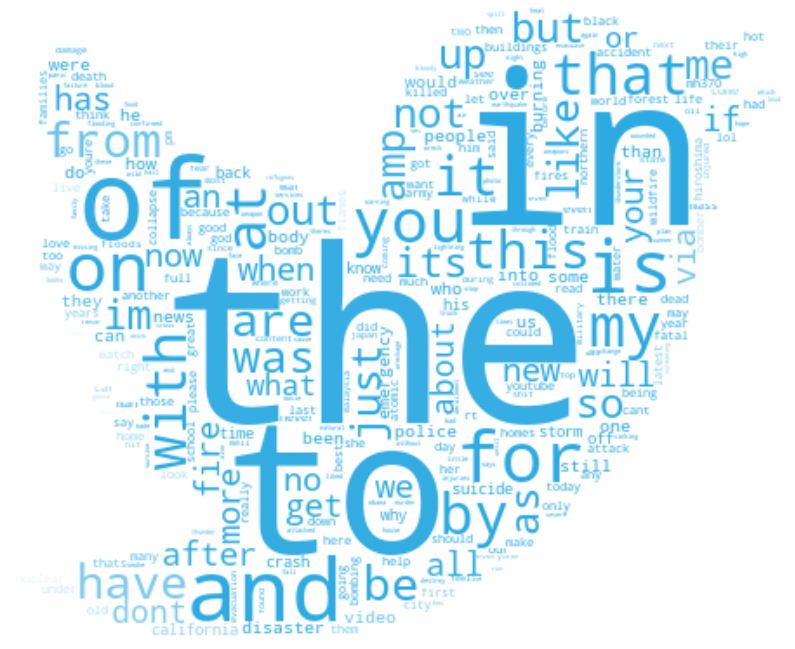
\includegraphics[width=1\textwidth]{graficos/Analisis Lexico Grafico/PalabrasMasUsadasSinFiltro.png}
    \caption{Logo de Twitter}
    \end{figure}
    
    Es importante destacar que en esta última visualización el tamaño de la palabra es proporcional al número de repeticiones de la misma.
    
    Luego, el siguiente gráfico es similar al anterior pero filtrando las preposiciones y artículos. El resultado se muestra continuación:
    
    \begin{figure}[H]
    \centering
    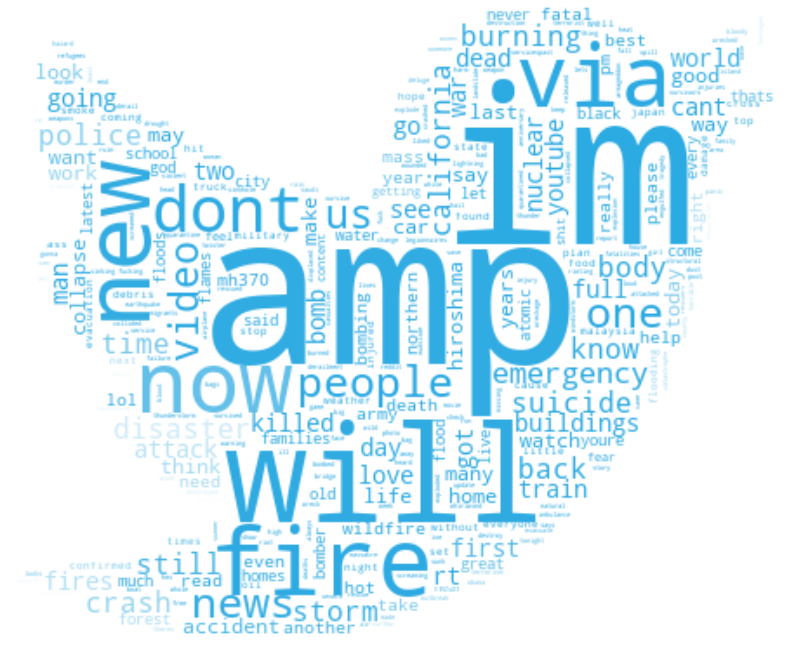
\includegraphics[width=1\textwidth]{graficos/Analisis Lexico Grafico/PalabrasMasUsadasConFiltro.png}
    \caption{Logo de Twitter}
    \end{figure}
    
    Habiendo estudiado el contenido de los \textit{Tweets} en términos de palabras y prolongación, resultó de gran interés observar la relación de estos campos con los \textit{Tweets} que tratan sobre un desastre real y aquellos que no lo hacen (aspecto que se considera como veracidad o \textit{Target}).
    
    \subsection{Relación entre el uso de palabras y la veracidad de \textit{Tweet}}
    En esta sección se prosigue a estudiar la veracidad y su relación con el uso de determinadas palabras. 
    
    Se comienza esta sección analizando la veracidad global de los \textit{Tweets} como se muestra en la siguiente visualización:
    
    \begin{figure}[H]
    \centering
    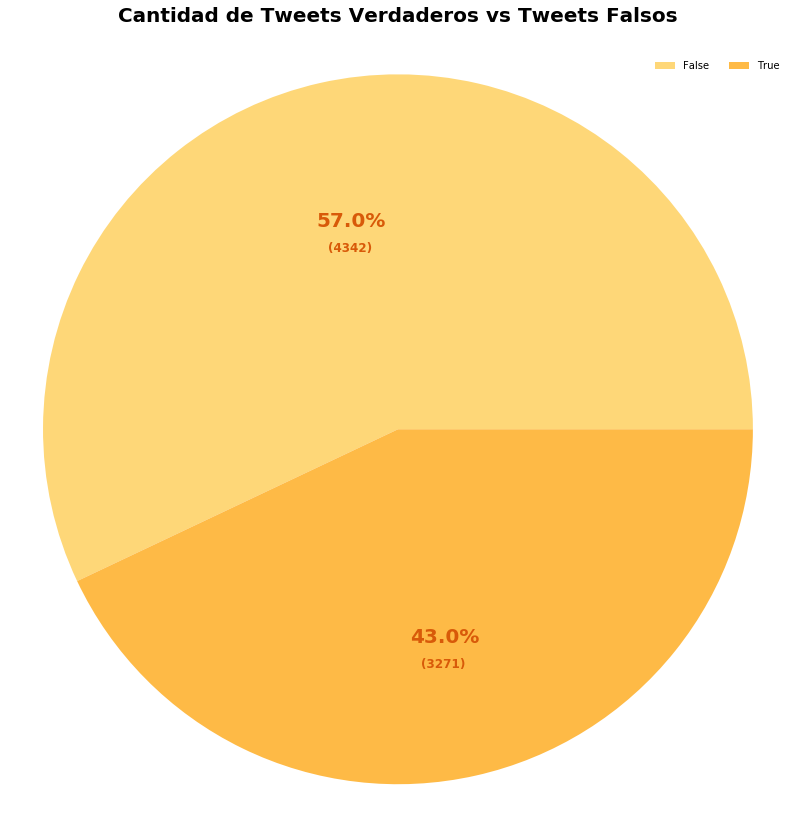
\includegraphics[width=1\textwidth]{graficos/Analisis Lexico Grafico/cantidad_de_tweets_verdadeos_vs_falsos.png}
    \end{figure}
    
    En un primer acercamiento a la veracidad de los \textit{Tweets}, se puede apreciar que la mayoría de éstos no hacen referencia a ningún tipo de desastre/accidente. A pesar de ello, es destacable que dentro del set de datos la cantidad de \textit{Tweets} para ambos casos es bastante pareja pues presentan una diferencia de 1071 \textit{Tweets}, en términos absolutos, y de 14\%, en términos relativos.
    
    Con ésto observado, se puede proceder a buscar relaciones entre la veracidad de los \textit{Tweets} y los distintos aspectos del texto de los mismos.
    
    El primer análisis que se efectúa tiene como objetivo el poder identificar si existe una conexión entre la frecuencia con la que se repiten las palabras y la veracidad promedio de los \textit{Tweets}  que las contienen. A modo de definición, se entiende como la veracidad de una palabra a la relación entre la cantidad total de veces que aparece ésta en distintos \textit{Tweets} y las que aparece en \textit{Tweets} que efectivamente refieren a un desastre.
    
    \begin{figure}[H]
    \centering
    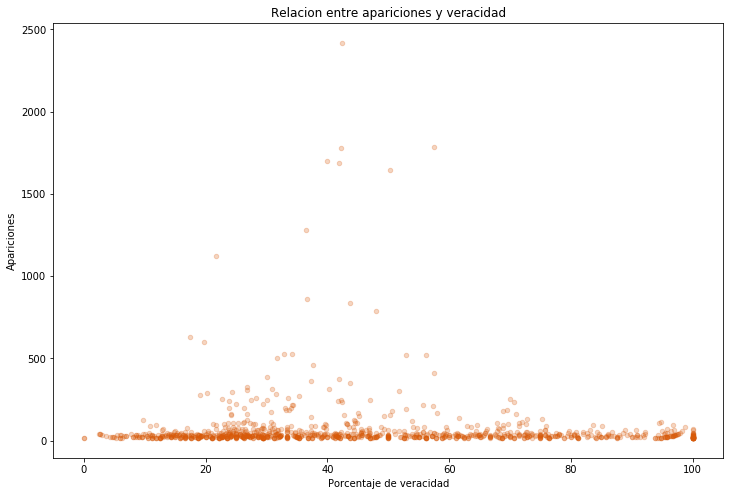
\includegraphics[width=1\textwidth]{graficos/Analisis Lexico Grafico/relacion_entre_apariciones_y_veracidad_2.png}
    \caption{} 
    \end{figure}
    
    Como se puede observar en este gráfico de dispersión, hay muy pocas palabras que aparecen mas de 500 veces, y dichas palabras tienen una veracidad cerca de la media. Por lo tanto no tienen impacto en un análisis relacionado a desastres. Es importante aclarar que si una apalabra aparece mas de una vez en el mismo \textit{Tweet}, esto de todas formas es considerado como una sola aparición de dicha palabra.
    
    Posteriormente, se prosigue a filtrar por palabras que aparecen menos de 500 veces. 
        
    \begin{figure}[H]
    \centering
    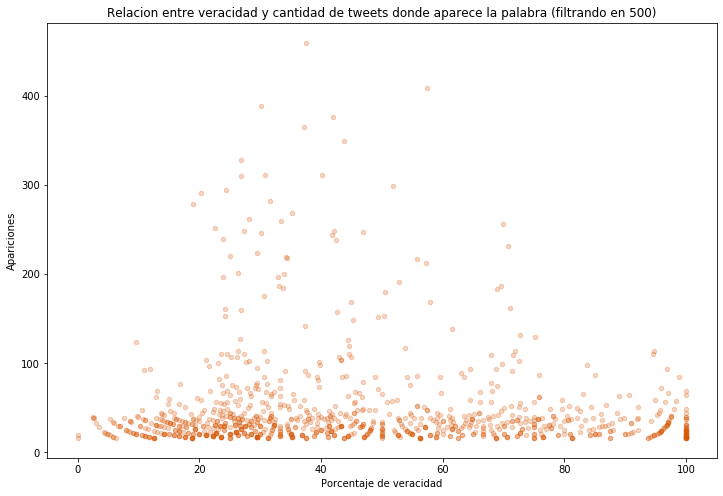
\includegraphics[width=1\textwidth]{graficos/Analisis Lexico Grafico/relacion_entre_apariciones_y_veracidad_filt_500.png}
    \caption{}   
    \end{figure}
    
    Al igual que en el gráfico anterior, se puede seguir observando que pasando las 100 apariciones no se encuentran palabras que tengan una veracidad atractiva.
    
    \begin{figure}[H]
    \centering
    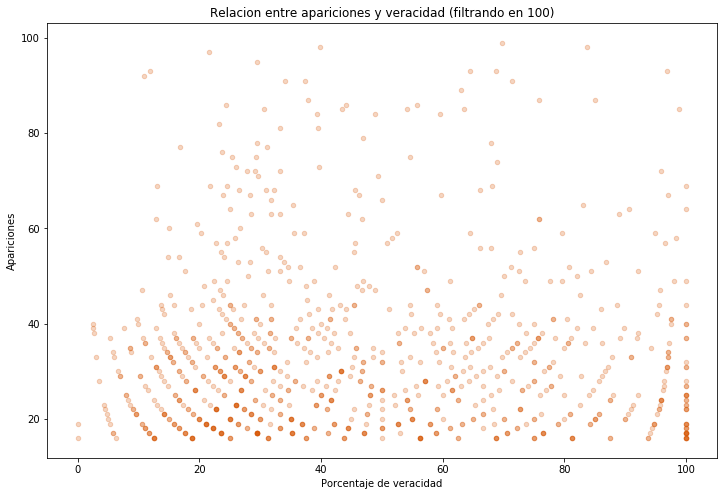
\includegraphics[width=1\textwidth]{graficos/Analisis Lexico Grafico/relacion_entre_aparicion_y_veracidad_filt_100.png}
    \caption{}
    \end{figure}
    
    En este gráfico se pueden observar cuestiones muy interesantes. Lo primero es que las palabras con mas apariciones tienden a rondar la media de veracidad, por lo tanto tienen poco impacto en un análisis del \textit{Target}.
    Por otro lado se pueden observar con claridad unas curiosas curvas, esto es debido a que el porcentaje de veracidad asociado a una palabra se calcula como el cociente entre apariciones veraces y apariciones totales. Siendo el eje vertical del gráfico las apariciones totales y el eje horizontal el porcentaje de veracidad, esto genera una relación de \texttt{ y = 1/x } entre ambas variables.
    También se puede apreciar una agrupación de muchas palabras en 100\% de veracidad, esto puede deberse a que la muestra no es suficientemente grande y hay palabras que solo aparecen en \textit{Tweets} verdaderos. Cuando en la realidad puede que no sea así.
    
    Un análisis que puede resultar aún mas interesante consiste en encontrar cuales son las palabras con mayor veracidad asociada, es decir las que suelen aparecer mucho más en \textit{Tweets} que hablan sobre desastres que en \textit{Tweets} que no lo hacen. En la visualización a continuación se procede a mostrar las palabras que solo aparecen en \textit{Tweets} veraces, cabe destacar que se decidido no mostrar las palabras que tienen menos de un 0.2\% de ocurrencias (aparecer en 12 \textit{Tweets} como mínimo para nuestro caso dado el tamaño del set). La razón de este filtro es evitar que aparezcan palabras que puedan llegar a tener alto o bajo porcentaje de veracidad solo por aparecer pocas veces (\textit{outliers}).
    
 
    \begin{figure}[H]
    \centering
    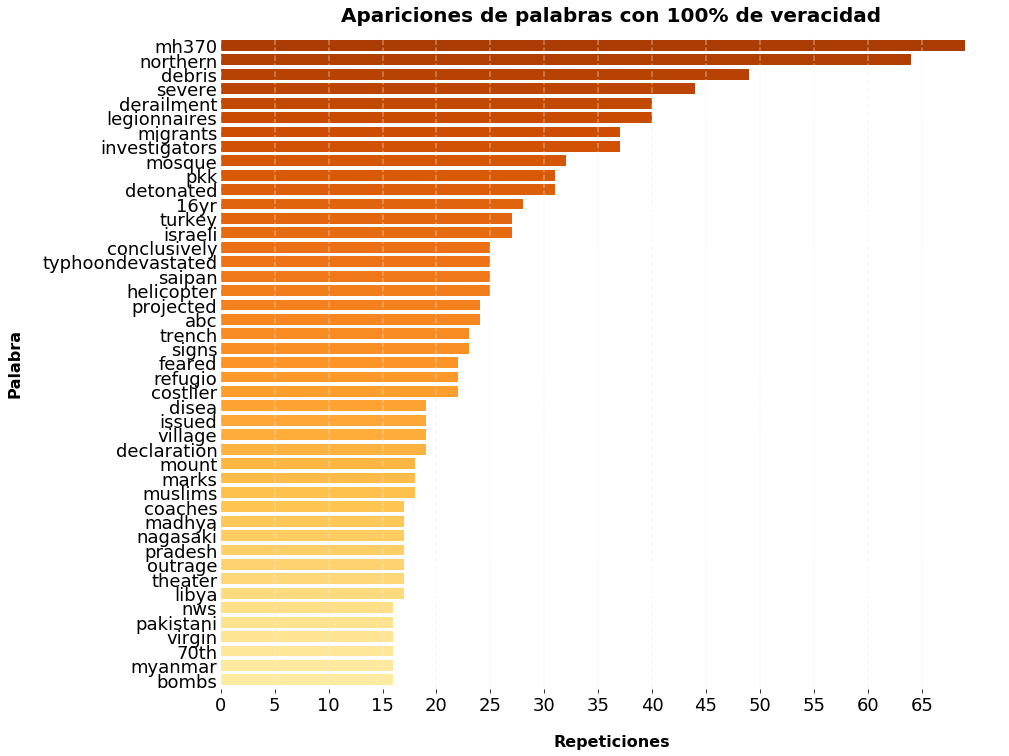
\includegraphics[width=1\textwidth]{graficos/Analisis Lexico Grafico/aparaciones_de_palabras_con_100_de_veracidad.png}
    \caption{Palabras 100\% veraces (Siempre que aparecen el \textit{Tweet} es verdadero)}
    \end{figure}
    
    Se aprecia que la palabra con mayor cantidad de repeticiones que aparece solo en \textit{Tweets} verídicos es ''mh370'', esta hace referencia al vuelo 370 de la aerolínea Malaysia Airlines que desapareció por causas desconocidas el día 8 de Marzo del 2014. Esto es razonable debido a que fue un accidente que tuvo una gran difusión mediática. El resto de palabras están también altamente relacionadas con desastres, lo cual era de esperar. 
    
    Para una mayor exhibición, en el siguiente gráfico se pueden observar aquellas palabras cuyas apariciones en \textit{Tweets} rondan entre el 90 y 100\% de veracidad. El tamaño de cada una está relacionado con la cantidad de repeticiones (teniendo en cuenta convención mencionada previamente) y el color, como indica la barra inferior del gráfico, está relacionado con el porcentaje de veracidad del total de \textit{Tweets} que las contenían.
    \begin{figure}[H]
    \centering
    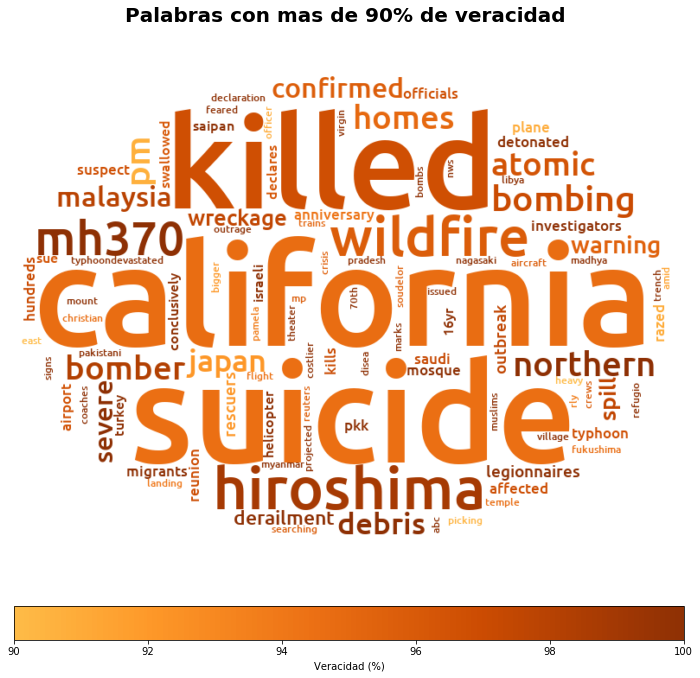
\includegraphics[width=1\textwidth]{graficos/Analisis Lexico Grafico/palabras_con_mas_de_90_de_veracidad.png}
    \caption{} 
    \end{figure}
    
    Como contraposición a las palabras con mayor índice de veracidad se pueden estudiar aquellas que sean completamente lo opuesto, es decir, las palabras cuyo porcentaje de veracidad en relación al total de \textit{Tweets} en los que aparecen es muy bajo. 
    
    
    \begin{figure}[H]
    \centering
    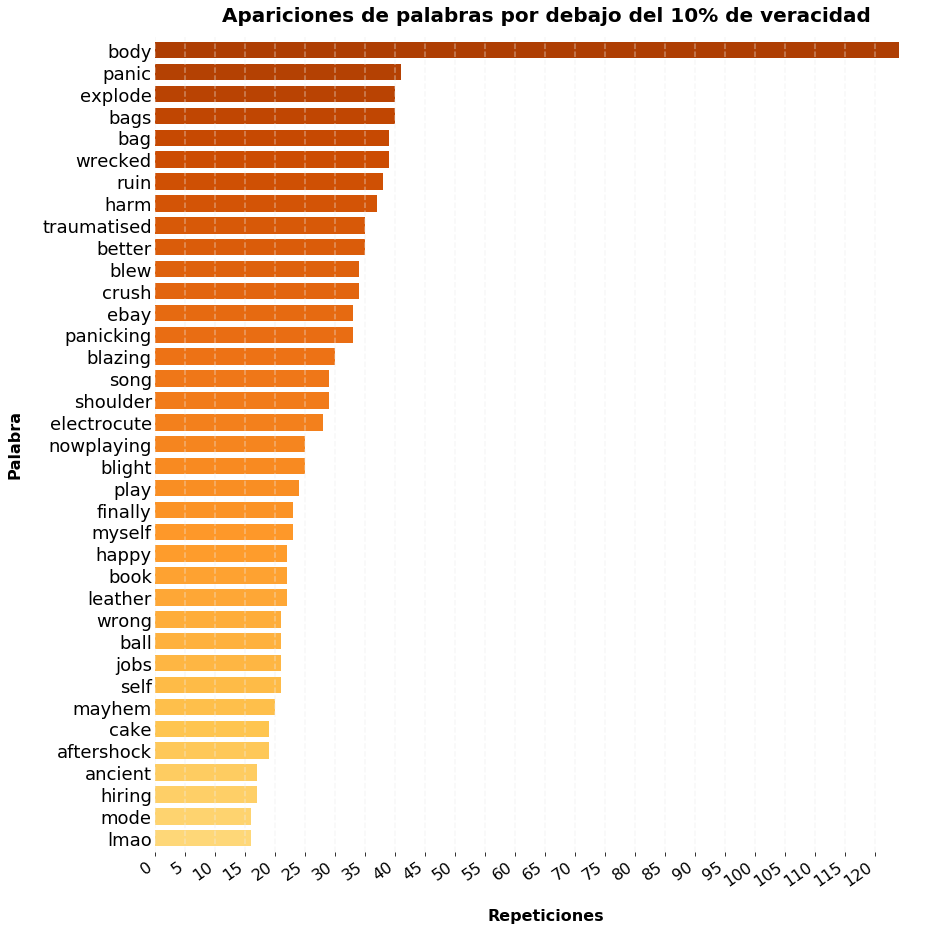
\includegraphics[width=1\textwidth]{graficos/Analisis Lexico Grafico/apariciones_de_palabras_por_debajo_de_10_de_veracidad.png}
    \caption{} 
    \end{figure}
    Como se puede apreciar y en contraste con lo dicho  para palabras con alto porcentaje de veracidad, las palabras con menos de 10\% de veracidad están en su mayoría poco relacionadas a un lenguaje esperable al hablar de una tragedia como por ejemplo \textit{``cake''}, \textit{``ebay''} o \textit{``song''}. Otras palabras mayormente relacionadas con tragedias que se encuentran en este gráfico podría deberse al uso coloquial que se les da y el cual no esta relacionado necesariamente con un desastre (por ejemplo, la palabra \textit{``crush''} en un \textit{Tweet} podría hacer referencia a un siniestro automovilístico o bien a un interés romántico de la persona que lo redactó).
    

    En un intento de estudiar el conjunto de datos de una manera más minuciosa, podemos quedarnos solo con las palabras que tienen menos de un 5\% de veracidad. Esto quiere decir que solamente en un  5\% de los casos en las cuales un \textit{Tweet} contiene esta palabra, el mismo es veraz. 
    
    \begin{figure}[H]
    \centering
    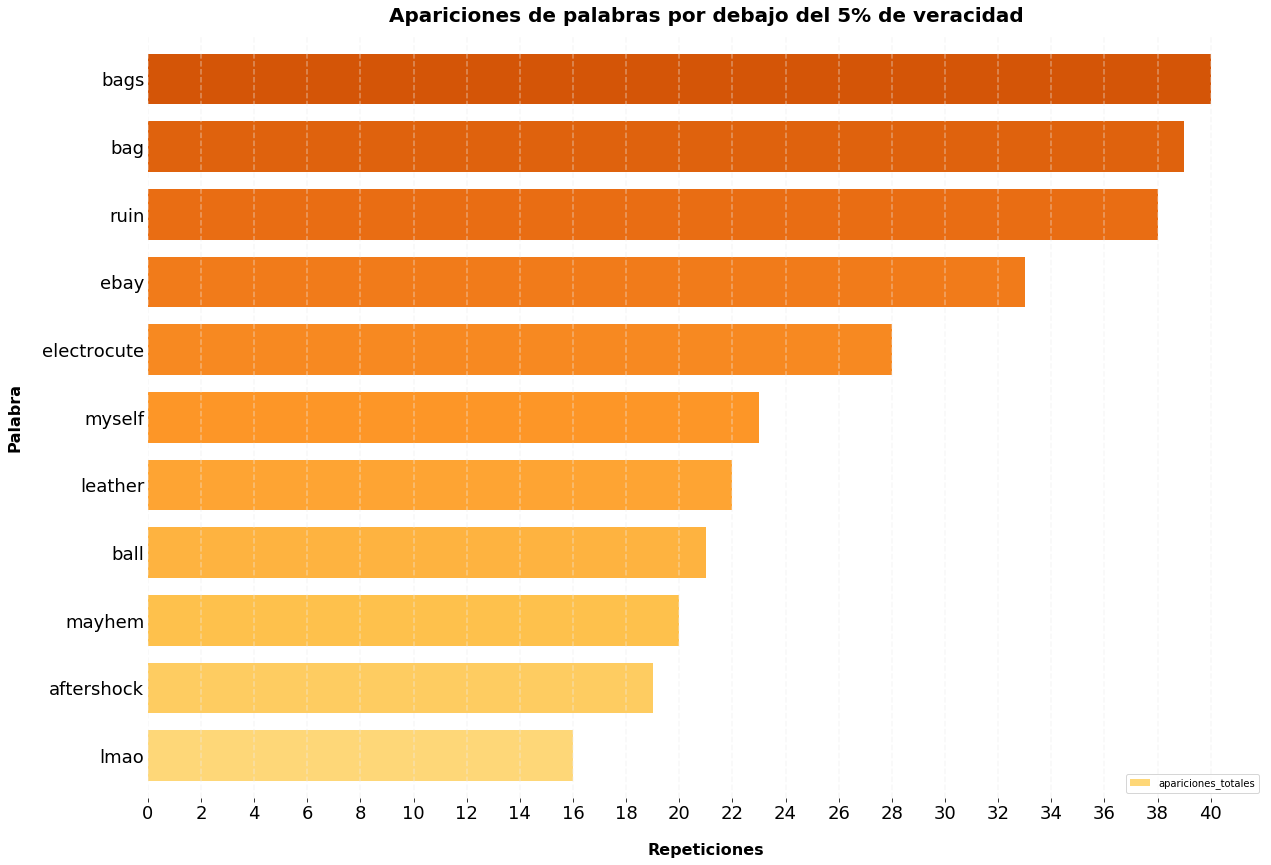
\includegraphics[width=1\textwidth]{graficos/Analisis Lexico Grafico/apariciones_de_palabras_por_debajo_de_5_de_veracidad.png}
    \caption{} 
    \end{figure}
    
    Se procede a hacer lo mismo pero para palabras que siempre que aparecen en un \textit{Tweet}, éste resultó no estar relacionado a ningún desastre.
    
    \begin{figure}[H]
    \centering
    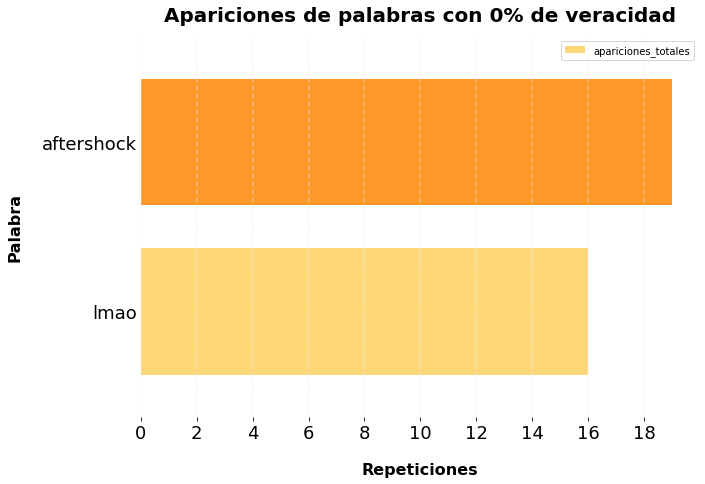
\includegraphics[width=0.6\textwidth]{graficos/Analisis Lexico Grafico/aparaciones_de_palabras_con_0_de_veracidad.png}
    \caption{} 
    \end{figure}
    
    De las dos palabras, una de ellas \textit{``lmao''}, la cual es propia de una conversación  coloquial y poco seria pues significa ``Partiéndose de Risa'' que evidentemente no es una expresión apropiada al estar refiriéndose a un desastre.
    
    La otra palabra es \textit{``aftershock''}, cuyo significado más inmediato al español es réplica, el cual sí esta asociado a un desastre. El hecho de que esta palabra no aparezca en ningún \textit{Tweet} relacionado a un desastre se puede deber a que el set de datos no es lo suficientemente grande.
    
    Análogamente al caso de las palabras con mayor veracidad, se procede a exponer las palabras que tienen menos de 10\% de veracidad en el   siguiente \textit{Word Cloud} :
    
     \begin{figure}[H]
    \centering
    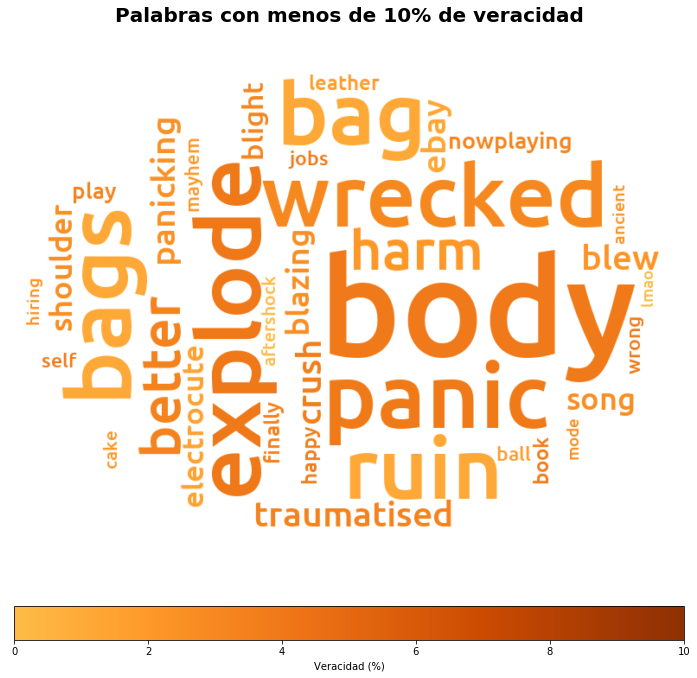
\includegraphics[width=1\textwidth]{graficos/Analisis Lexico Grafico/palabras_con_menos_de_10_de_veracidad.png}
    \caption{} 
    \end{figure}
    
    Al haber estudiado aquellas palabras con mayor y menor porcentaje de veracidad, es propicio observar cómo se comporta las distribución de palabras en relación a éste aspecto.
    
    \begin{figure}[H]
    \centering
    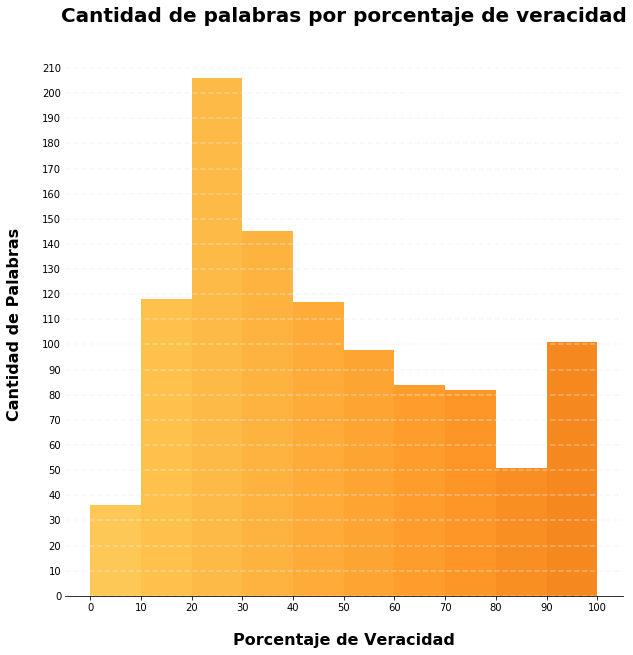
\includegraphics[width=1\textwidth]{graficos/Analisis Lexico Grafico/cantidad_de_palabras_por_porcentaje_de_veracidad.png}
    \caption{}
    \end{figure}

    La cantidad de palabras que tienen un porcentaje de veracidad elevado (mayor al 80\%), conforman una pequeña parte con respecto al total. Esto es lógico si se tiene en cuenta que las palabras con veracidad elevada son a menudo las que pertenecen al vocabulario o familia de palabras empleadas cuando se busca hablar o dar información acerca de un accidente o desastre. El pico que se observa para valores entre  20\% y  40\% puede deberse al uso de un lenguaje más informal que predomina en la red social y que si bien puede tratar sobre desastres también, es la forma usual de comunicación de una importante cantidad de usuarios de la plataforma, y al tener el set de datos una mayor cantidad de \textit{Tweets} ``falsos'', es esperable que dicho pico este en un punto más bajo que el 50\%. 
    
    \subsection{Estudio de la longitud de los \textit{Tweets}}

    Con el objetivo de profundizar aún más, se puede agregar una variable más al estudio de la veracidad, tal como la prolongación de los \textit{Tweets} tanto en palabras como caracteres. De esta manera, se elaboraron las siguientes visualizaciones.

    \begin{figure}[H]
    \centering
    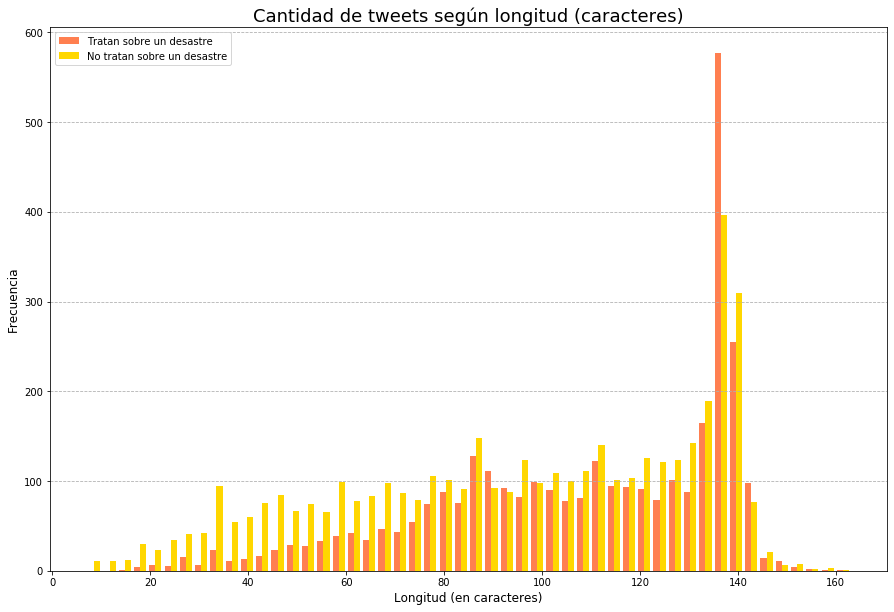
\includegraphics[width=1\textwidth]{graficos/Analisis Lexico Grafico/cantidad_de_tweets_segun_longitud_en_caracteres.png}
    \caption{}
    \end{figure}
    
    Como se puede observar, hay una marcada diferencia en la distribución de los \textit{Tweets} según su longitud en caracteres. Se observa que los \textit{Tweets} que efectivamente refieren a desastres tienden a ser mas largos que los que no. Esto puede deberse a que las personas que escriben estos \textit{Tweets} tienden a querer aportar la mayor cantidad de información posible sobre el mismo, con una considerada cantidad de detalles. Con lo cual seria lógico que estos resulten más extensos.
    
    Por otro lado, se observa que dentro de los \textit{Tweets} de menor cantidad de caracteres suelen prevalecer los falsos. Esto es esperable siguiendo el razonamiento previamente explicado.
    
    Algo que puede ser de interés es analizar la veracidad de los \textit{Tweets} según la cantidad de palabras que contienen.
    
    \begin{figure}[H]
    \centering
    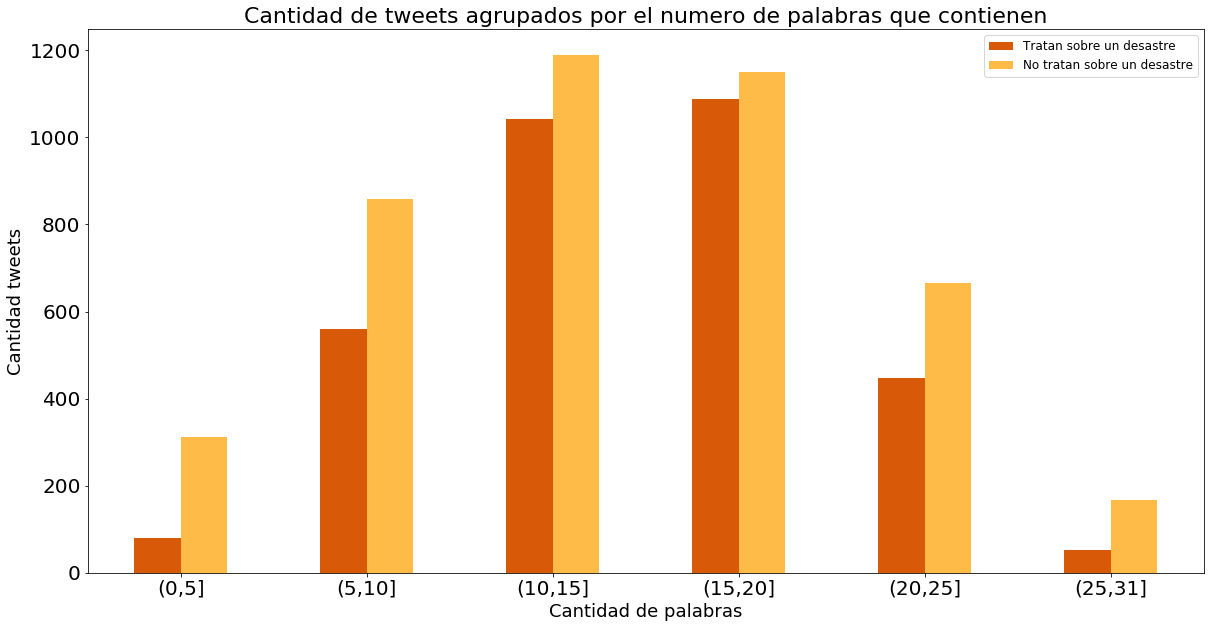
\includegraphics[width=1\textwidth]{graficos/Analisis Lexico Grafico/cantidad_de_tweets_agrupados_por_numero_de_palabras.png}
    \caption{}
    \end{figure}
    
    El gráfico muestra que para cualquier grupo, la cantidad de \textit{Tweets} que hacen referencia a una tragedia es menor que la cantidad de \textit{Tweets} que no lo hacen. Además, en este gráfico no se observa el patrón del gráfico anterior; en este caso la cantidad de Tweets que no hacen referencia a un desastre siempre es mayor. En base a esto y que en el gráfico de caracteres si se puede observar una diferencia, podemos inferir que los \textit{Tweets} veraces tienden a usar palabras más largas.
    
    Se gráfica la longitud promedio de las palabras según a que tipo de \textit{Tweet} pertenecen. 
    
     \begin{figure}[H]
    \centering
    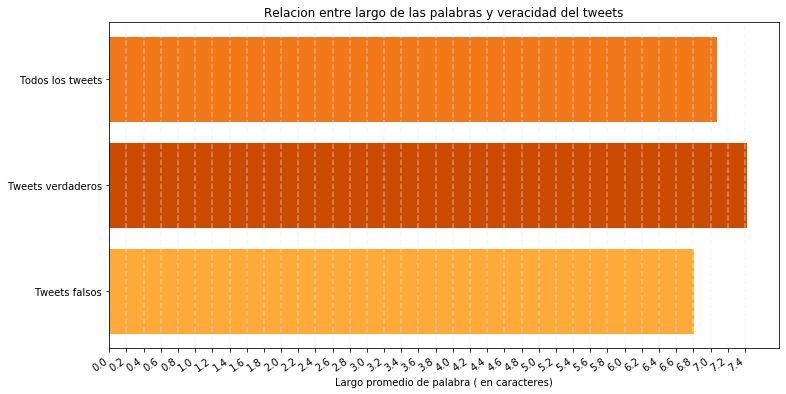
\includegraphics[width=1\textwidth]{graficos/Analisis Lexico Grafico/longitud promedio barras.png}
    \caption{}
    \end{figure}

    En este gráfico se puede observar efectivamente que los \textit{Tweets} veraces tienden a tener palabras más largas, lo cual confirma nuestra hipótesis previa.

   \subsection{Estudio de características especiales de los \textit{Tweets}}
    
    Finalmente, debido a que \textit{Twitter} es una red social que posee características propias con caracteres utilizados dentro de la plataforma que tienen funcionalidades tales como \textit{``\#''} (Hashtag, utilizado para hablar sobre algún tópico) o \textit{``@''} (para mencionar a otro usuario), se procedió a hacer un análisis de la relación existente entre la aparición estos caracteres específicos dentro de un \textit{Tweet} y la veracidad del mismo. Además, se agrega a este estudio la consideración de la existencia de símbolos lingüísticos usuales (\textit{¡, !, ¿, ?}), nombres de locaciones geográficas, direccionamientos a páginas web (\textit{URLs}) o el simple hecho de que el \textit{Tweet} comience con letra mayúscula, puesto que son casos particularmente interesantes de analizar en caso de que exista alguna tendencia.

    \begin{figure}[H]
    \centering
    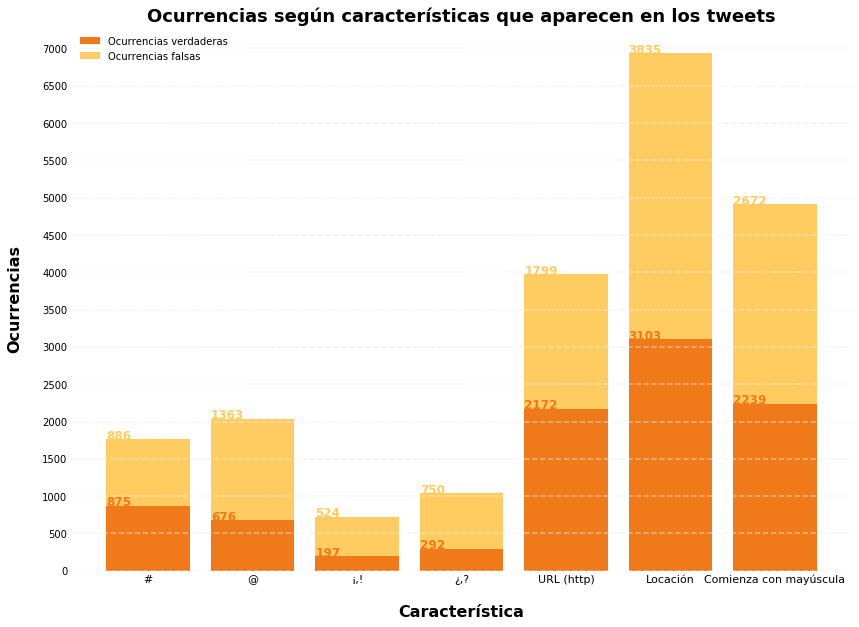
\includegraphics[width=1\textwidth]{graficos/Analisis Lexico Grafico/ocurrencias_segun_caracteristicas_que_aparecen_en_los_tweets.png}
    \caption{} 
    \end{figure}
    
    \begin{figure}[H]
    \centering
    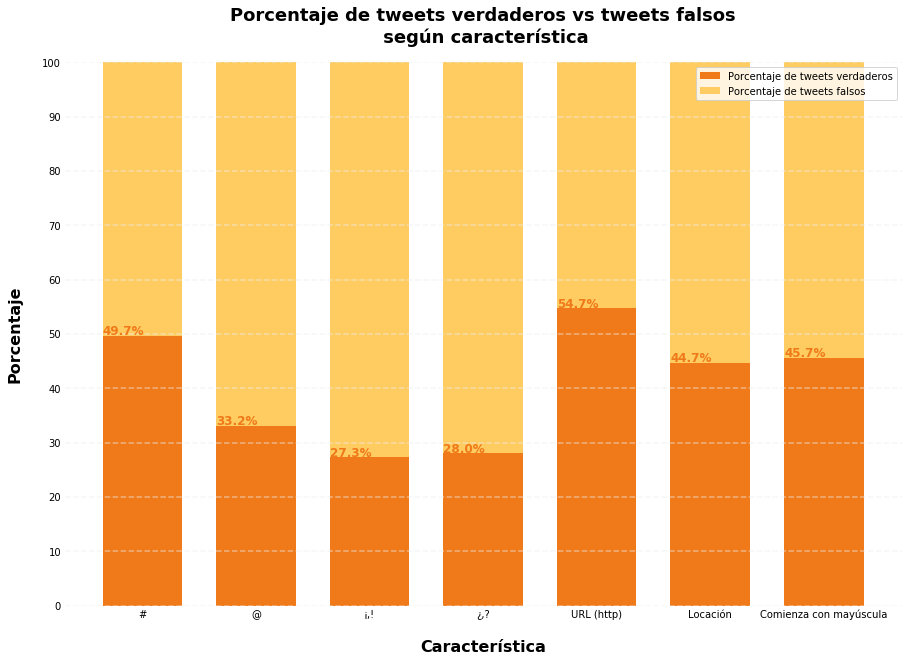
\includegraphics[width=1\textwidth]{graficos/Analisis Lexico Grafico/porcentaje_caracteristicas.png}
    \caption{} 
    \end{figure}
    
    Al examinar los resultados obtenidos se puede afirmar que la presencia de \textit{``\#''}, \textit{URLs}, locaciones y mayúsculas como letra inicial no posee impacto en la veracidad de los \textit{Tweets}. Caso contrario es el observable en aquellos que incluyen signos de exclamación, interrogación y \textit{``@''} en su contenido, puesto que sólo alrededor de un tercio (27.3\%, 28\% y 33.2\%, respectivamente) de los \textit{Tweets} que contienen alguno de estos caracteres tratan sobre desastres reales. Esto se puede deber a que los medios formales de comunicación no utilizan estos caracteres para comunicar información sobre desastres u accidentes.
    
    Por otra parte, otro de los aspectos que se puede analizar frente a la presencia de estas características específicas es el de la longitud de los \textit{Tweets} que las poseen. Los siguientes dos gráficos representan los resultados obtenidos con dicho afán.

    \begin{figure}[H]
    \centering
    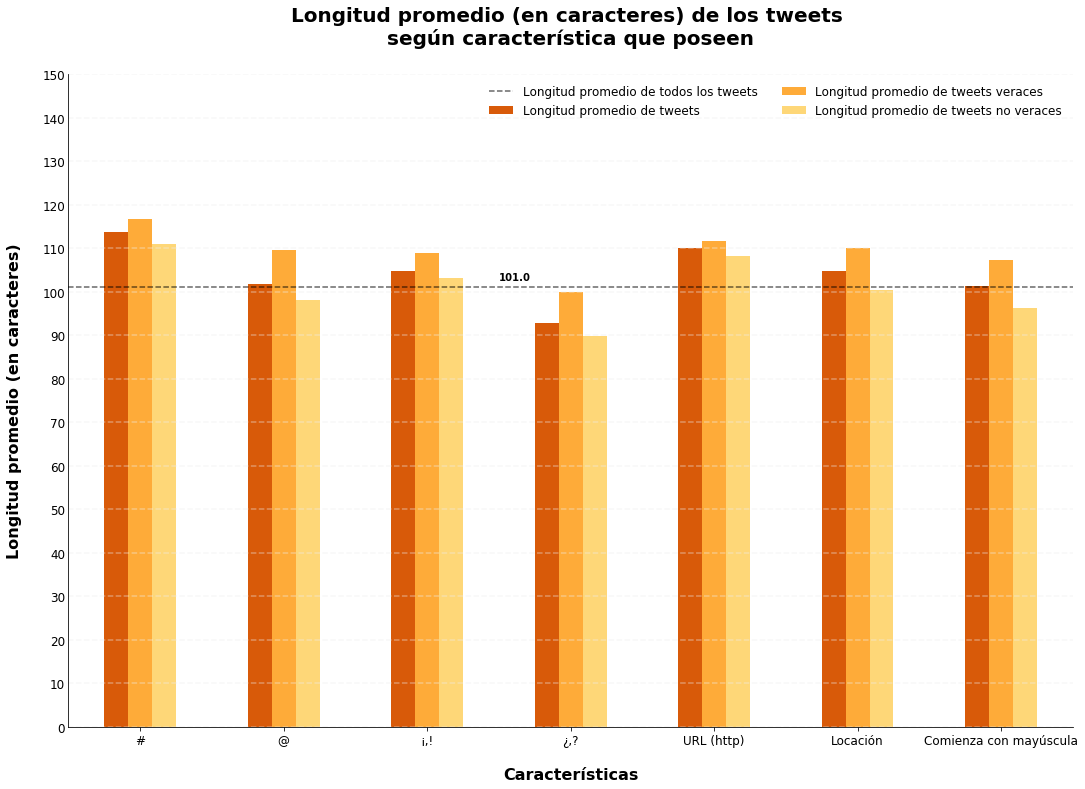
\includegraphics[width=.9\textwidth]{graficos/Analisis Lexico Grafico/long_promedio_char_tweets_segun_caracteristica.png}
    \caption{} 
    \end{figure}
    
    \begin{figure}[H]
    \centering
    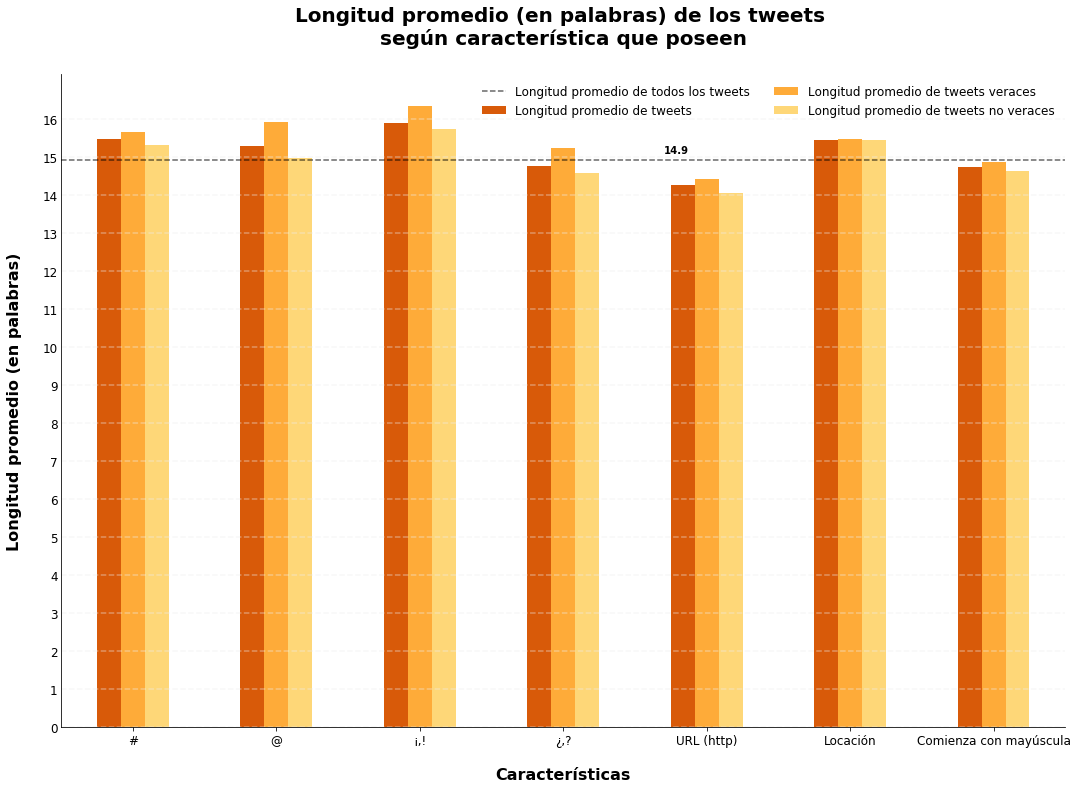
\includegraphics[width=.9\textwidth]{graficos/Analisis Lexico Grafico/long_prom_words_tweets_segun_caracteristicas.png}
    \caption{} 
    \end{figure}
    
    A partir de estas visualizaciones se puede observar una serie de leves tendencias. La primera, es que la prolongación promedio de los \textit{Tweets} veraces posee una ligera tendencia a ser mayor a la de los \textit{Tweets} que no tratan sobre desastre, ya sea en caracteres o palabras, sin importar la característica que posean.
    
    Por otro lado, la longitud en caracteres de aquellos \textit{Tweets} que contienen signos de interrogación es menor al promedio, al igual que la extensión en palabras de aquellos \textit{Tweets} que contienen direcciones de enlace (\textit{URLs}). 
    
    Es notable que los \textit{Tweets} que poseen locación tienen la misma longitud promedio independientemente de su veracidad y esta se encuentra ligeramente sobre el promedio.  
    
    \newpage
    \section{Análisis de \textit{Keywords}}\label{sec:intro}

    Se continúa con el análisis de las \textit{Keywords} usadas en los \textit{Tweets}. Es relevante aclarar que para los análisis que prosiguen no se tendrán en cuenta todas las \textit{Keywords}, sólo se consideran aquellas que se encuentran asociadas a 29 o más \textit{Tweets}. Ésta decisión es tomada para evitar el problema de la sobre representación de aquellas cuya cantidad de repeticiones es considerablemente inferior en comparación al resto. 
    
    Para ello, en primera instancia se calcula el promedio de repetición de las 222 distintas \textit{Keywords} (a los \textit{Tweets} que no poseen \textit{Keyword} asociada, se les asigna 'none\_keyword'), obteniendo como resultado alrededor de 34 repeticiones por \textit{Keyword}. Sin embargo, recortar el espectro estudiado en este valor significa dejar fuera del análisis a alrededor del 35\% (77 \textit{Keywords}) del total. Por ello se opta por reducir la vara a 29, donde sólo 13 de ellas no son tenidas en cuenta y la distancia al valor promedio no es significativa. 
    
     \subsection{Relación entre el uso de \textit{Keywords} y la longitud de los \textit{Tweets}}
    
    Para comenzar se pretende estudiar la relación entre el uso de las distintas \textit{Keywords} con la prolongación del texto de los \textit{Tweets} asociados a ellas. Éste primer gráfico muestra la longitud promedio de los \textit{Tweets} agrupados por \textit{Keyword}. 

    \begin{figure}[H]
    \centering
    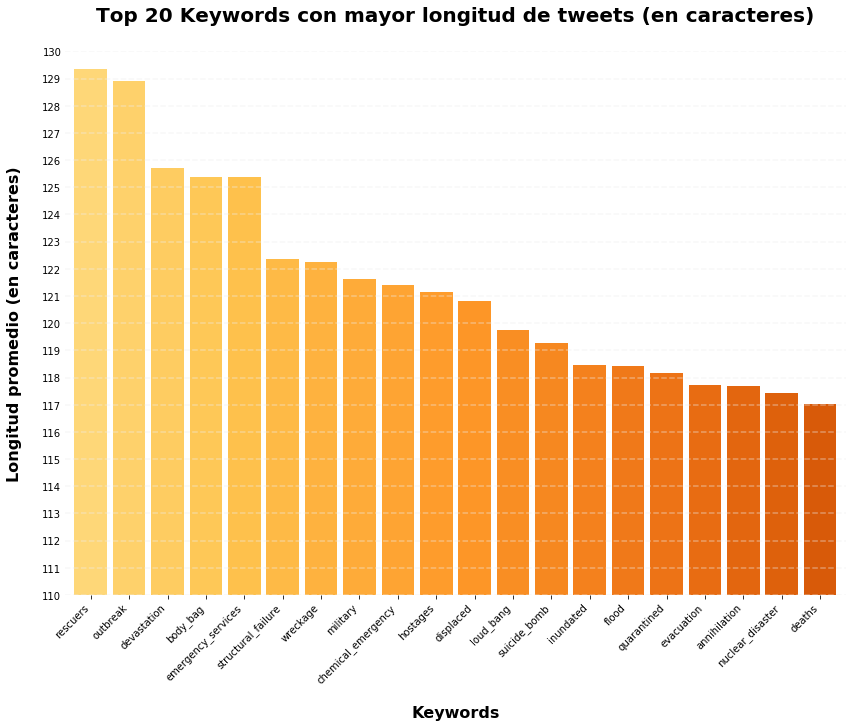
\includegraphics[width=1\textwidth]{graficos/Analisis de Keyword/top_20_long_con_mayor_long_de_tweets.png}
    \caption{} 
    \end{figure}
    
    Como se puede apreciar, las longitudes se acercan al límite de 140 caracteres por \textit{Tweet} que ofrece la plataforma, pues más de la mitad se encuentran sobre los 120 caracteres. 
    
    Si ahora se realiza un análisis similar modificando la manera en que se mide la longitud a palabras por \textit{Tweet}, se obtiene el siguiente gráfico:
    
    \begin{figure}[H]
    \centering
    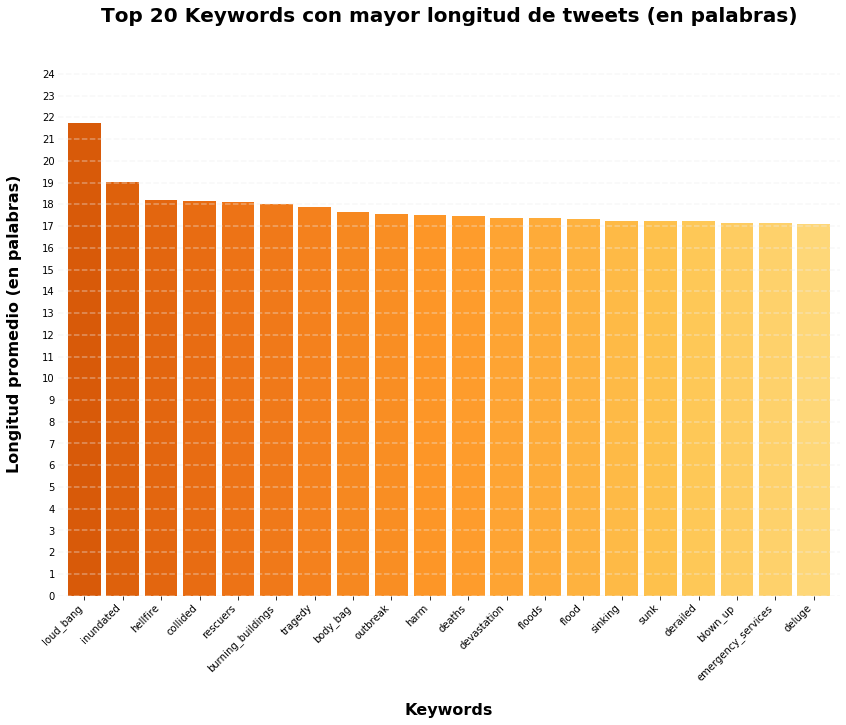
\includegraphics[width=1\textwidth]{graficos/Analisis de Keyword/top_20_keywords_con_mayor_long_de_tweets_en_palabras.png}
    \caption{} 
    \end{figure}
     
    Se puede observar que la mayoría de \textit{Keywords} corresponden a \textit{Tweets} que tienen como media entre 17 y 18 palabras.
    
    De forma análoga, se estudian las \textit{Keywords} que corresponden a \textit{Tweets} con menor longitud promedio en caracteres. 
    
    \begin{figure}[H]
    \centering
    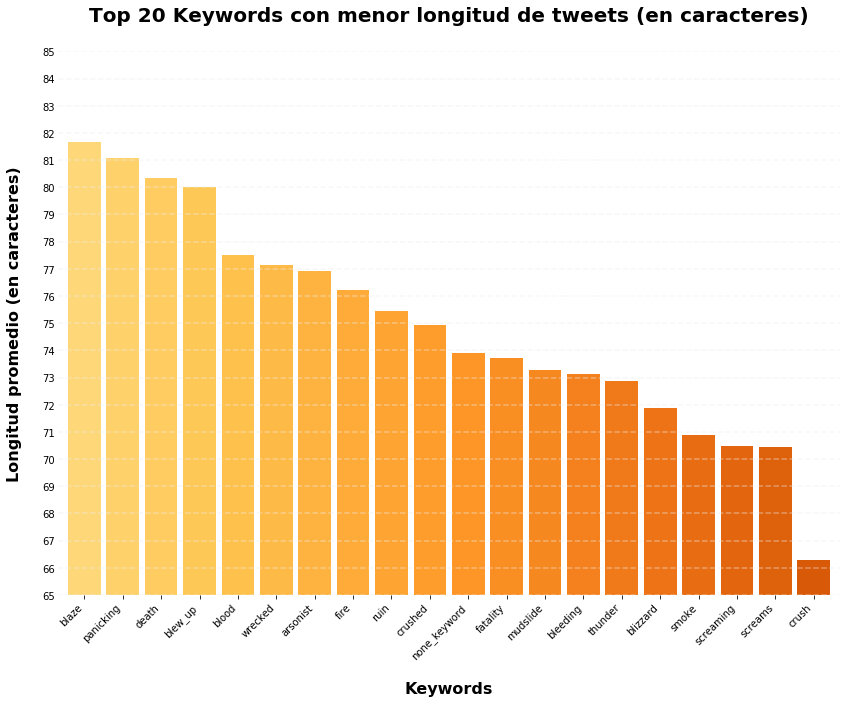
\includegraphics[width=1\textwidth]{graficos/Analisis de Keyword/top_20_keywords_con_menor_long_de_tweets_en_caracteres.png}
    \caption{} 
    \end{figure}
    
    Se puede observar claramente que la longitud promedio mínima está ligeramente por encima los 66 caracteres. Además, comparado con las \textit{Keywords} con mayor longitud en caracteres, hay una diferencia notable. 
    
    Ahora, midiendo la longitud en palabras, se obtiene el siguiente gráfico:
    \begin{figure}[H]
    \centering
    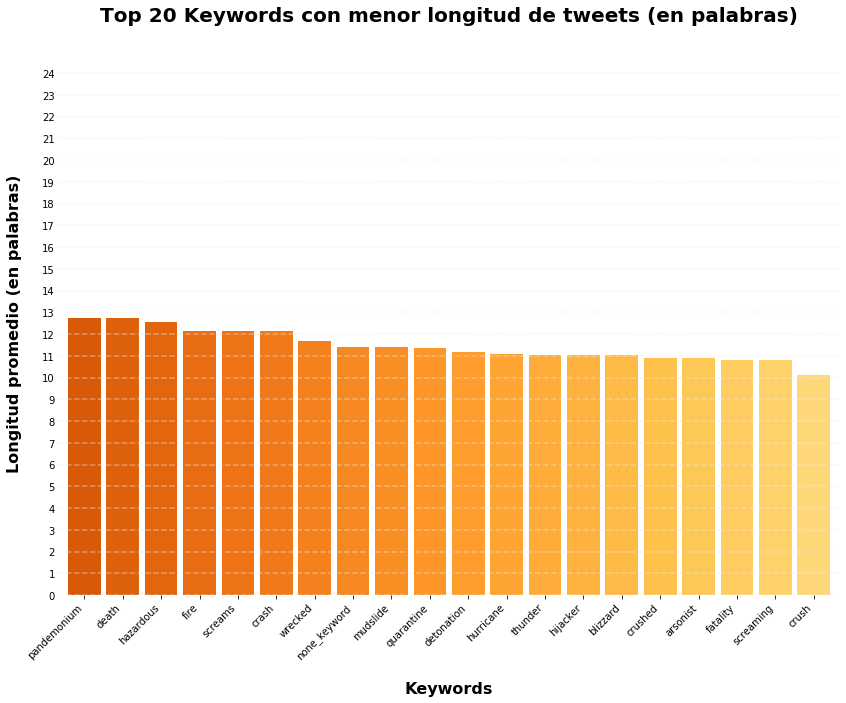
\includegraphics[width=1\textwidth]{graficos/Analisis de Keyword/top_20_keywords_con_menor_long_de_tweets.png}
    \caption{} 
    \end{figure}
    Se observa que la longitud promedio mínima esta sobre las 10 palabras. También se puede ver que comparado con las \textit{Keywords} con mayor longitud en palabras, la diferencia de longitudes no es significativa. 
    
    Como conclusión de las últimas visualizaciones se puede afirmar que no existe ninguna relación aparente entre la prolongación del \textit{Tweet} y la \textit{Keyword} asociada a este. Esto se debe a que ninguno de los grupos de \textit{Keywords} representadas en cada gráfico presentan rasgos que los distingan del resto, todos se relacionan a algún tipo de desastre (sin importar la naturaleza del mismo).
    
    \subsection{Relación entre el uso de \textit{Keywords} y la veracidad de los \textit{Tweets}}
    
    De manera análoga a la sección anterior, una parte de gran interés del análisis exploratorio relacionado con las \textit{Keywords} llega cuando se agrega al estudio el porcentaje de veracidad del total de \textit{Tweets} asociados a un mismo \textit{Keyword}.    
    
    Como visualización inicial se procede a mostrar aquellos \textit{Keywords} asociados a los grupos de \textit{Tweets} con mayor grado de veracidad promedio.
    
    \begin{figure}[H]
    \centering
    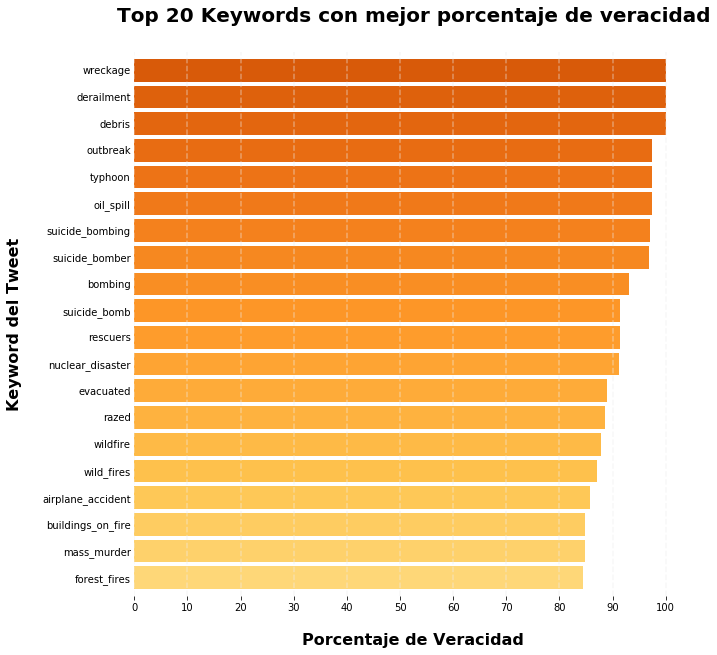
\includegraphics[width=1\textwidth]{graficos/Analisis de Keyword/top_10_keywords_con_mejor_porcentaje_de_veracidad.png}
    \caption{} 
    \end{figure}
    
    Como se observa, gran parte de las \textit{Keywords} pertenecen o tienen una relación estrecha con el conjunto/familia de palabras que son empleadas a menudo para describir o dar información acerca de accidentes o desastres. Asimismo muchas de estas difícilmente podrían ser empleadas en cualquier otro tipo de contexto o situación, y es, probablemente, por esa razón que presentan tan elevada veracidad. Tal es el caso de palabras como ``derailment'', la cual significa descarrilamiento, o ``debris'', escombros. Ambas \textit{Keywords} se encuentran entre las de mayor veracidad y sus significados pueden ser considerados muy puntuales, corroborando la explicación anterior. 
    
    En contraposición a estas \textit{Keywords} se hallan aquellas cuya veracidad asociada es extremadamente pequeña y, a los fines de demostrar claramente las diferencias entre ambos casos, se enseñan a continuación preservando la escala de la última visualización.
    
    \begin{figure}[H]
    \centering
    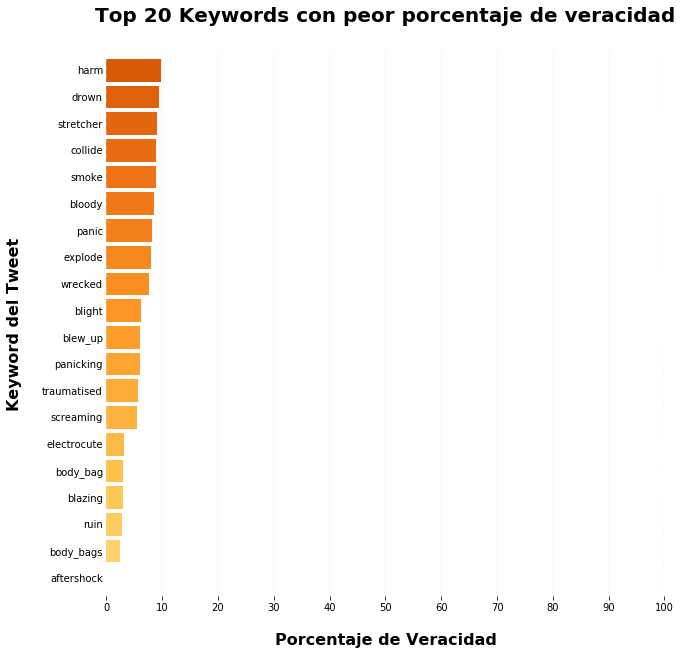
\includegraphics[width=1\textwidth]{graficos/Analisis de Keyword/top_20_keywords_con_peor_porcentaje_de_veracidad.png}
    \caption{} 
    \end{figure}
    
    A diferencia del anterior gráfico, estas \textit{Keywords} no pueden ser consideradas ``exclusivas'' del conjunto de palabras frecuentemente utilizadas para referirse a desastres/accidentes. Son palabras de las cuales se puede hacer uso en contextos muy diversos completamente diferentes a los concernientes a este trabajo y es por esa razón que tienen tan baja veracidad (<10\%). Por ejemplo, \textit{``smoke''} significa humo, \textit{``ruin''} se traduce como ruina y \textit{``screaming''}, gritando. Éstas palabras pueden ser utilizadas en diversos contextos para múltiples situaciones no necesariamente relacionadas con algún desastre.  
    
    
    \subsection{Análisis de frecuencia de aparición de las \textit{Keywords}}
    Si bien ahora se conocen las \textit{Keywords} con mayor y menor grado de veracidad, resulta atractivo poder visualizar cuáles de ellas se encuentran entre las de mayor y menor cantidad de \textit{Tweets} asociados. Para lograr esto, en primer lugar se grafican las 10 \textit{Keywords} con mayor y con menor frecuencia de aparición.
    \begin{figure}[H]
    \centering
    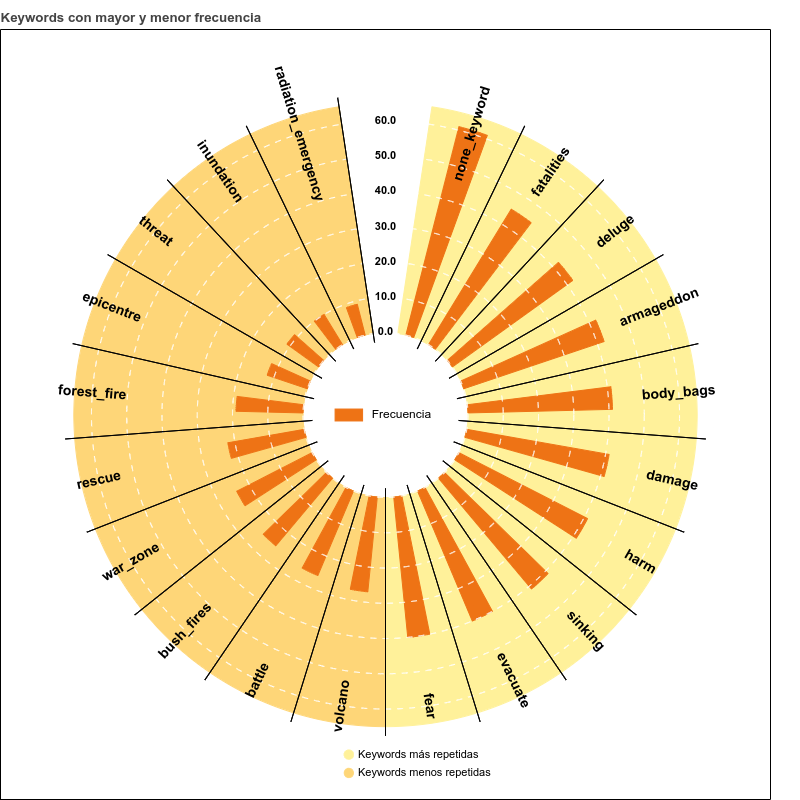
\includegraphics[width=1\textwidth]{graficos/Analisis de Keyword/rosquete_keywords_repetidas.png}
    \caption{} 
    \end{figure}
    
    A partir de esta información se puede proceder a vincular los datos sobre veracidad asociada a un \textit{Keyword} y la cantidad que veces que aparece. El producto de esto se ve representado en la \textit{wordcloud} que se enseña a continuación. Cabe destacar que, de igual manera que en los anteriores gráficos de este estilo, cuanto mayor sea la frecuencia de una palabra, mayor será el tamaño de esta en la visualización.
    
    \begin{figure}[H]
    \centering
    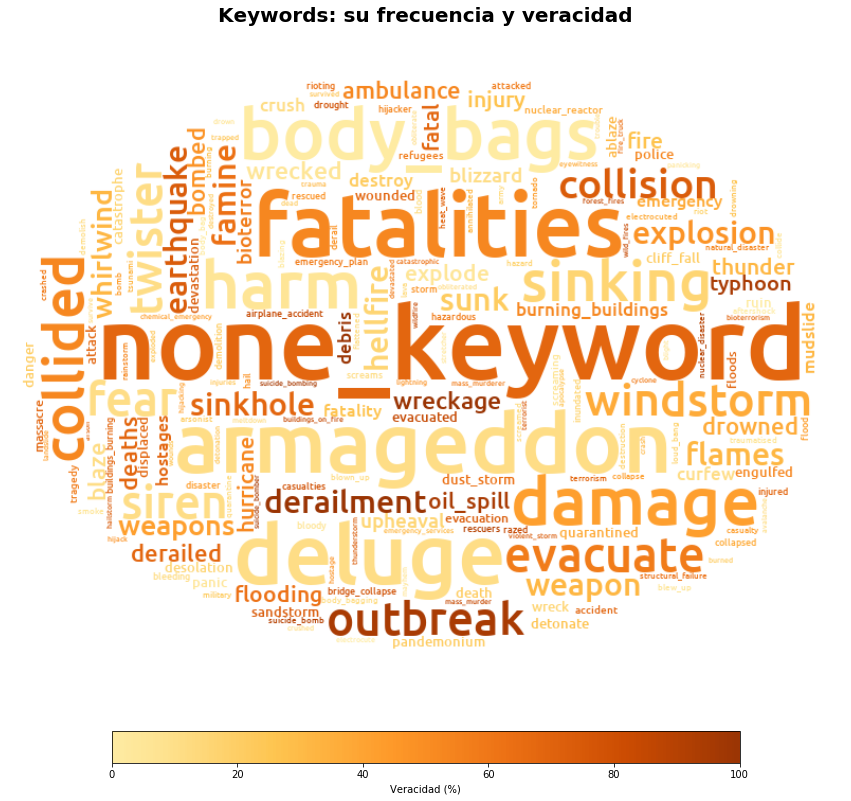
\includegraphics[width=1\textwidth]{graficos/Analisis de Keyword/keywords_frec_y_veracidad.png}
    \caption{} 
    \end{figure}
    
    Por medio de este gráfico se puede apreciar que una gran cantidad de Tweets no tienen una \textit{Keyword} asociada y que, además, éstos tienen un alto porcentaje de veracidad. Otras \textit{Keywords} destacables debido a su cantidad y porcentaje de veracidad son: \textit{``outbreak''}, \textit{``collision''}, \textit{``fatalities''} y \textit{``damage''}, lo cual tiene sentido ya que son palabras que se usan a menudo cuando se quiere hacer referencia a accidentes. 
    
    También cabe destacar que a pesar de tener \textit{Tweets} de varias partes del mundo, todas éstas \textit{Keywords} se encuentran en inglés, esto puede ser una mera coincidencia o dar cierto indicio de un tipo de sesgo al momento de recolectar los datos para el set. 
    
    \begin{figure}[H]
    \centering
    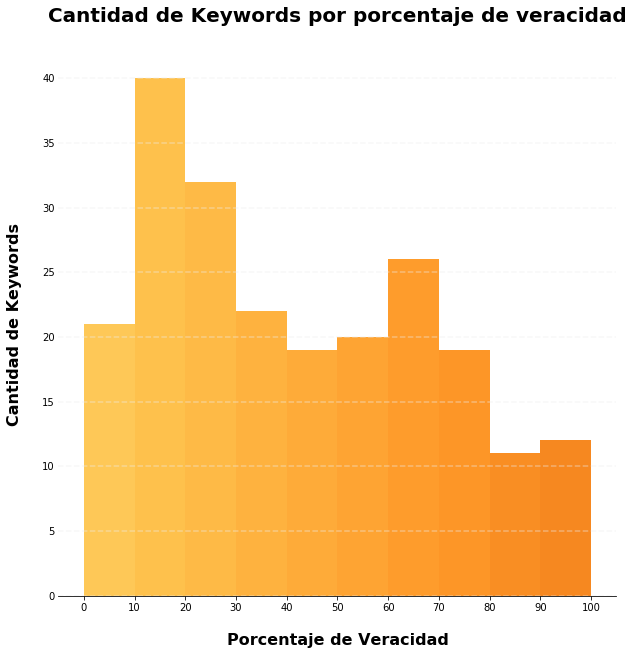
\includegraphics[width=1\textwidth]{graficos/Analisis de Keyword/cantidad_de_keywords_por_porcentaje_de_veracidad.png}
    \caption{} 
    \end{figure}
    
    Se puede apreciar que después del pico que se da entre el 10 y 20\% de veracidad donde se llega a 40 \textit{Keywords}, la cantidad de estas por porcentaje de veracidad comienza a bajar cuasi constantemente. A partir de esto se puede concluir que la mayoría de las \textit{Keywords} (más del 60\%) se hallan asociadas a grupos de \textit{Tweets} con un porcentaje de veracidad menor al 50\%.
        
    \subsubsection{Relación entre la veracidad de las \textit{Keywords} y la longitud promedio}
    
    Antes de comenzar el análisis del tema referido, es propicio verificar en primer lugar si se continúa manteniendo la relación lineal existente entre la longitud en palabras y caracteres de los \textit{Tweets}, pero en este caso agrupados por la \textit{Keyword} asociada a estos. En el siguiente \textit{Scatter Plot}, se grafica el comportamiento resultante obtenido:
    
    \begin{figure}[H]
    \centering
    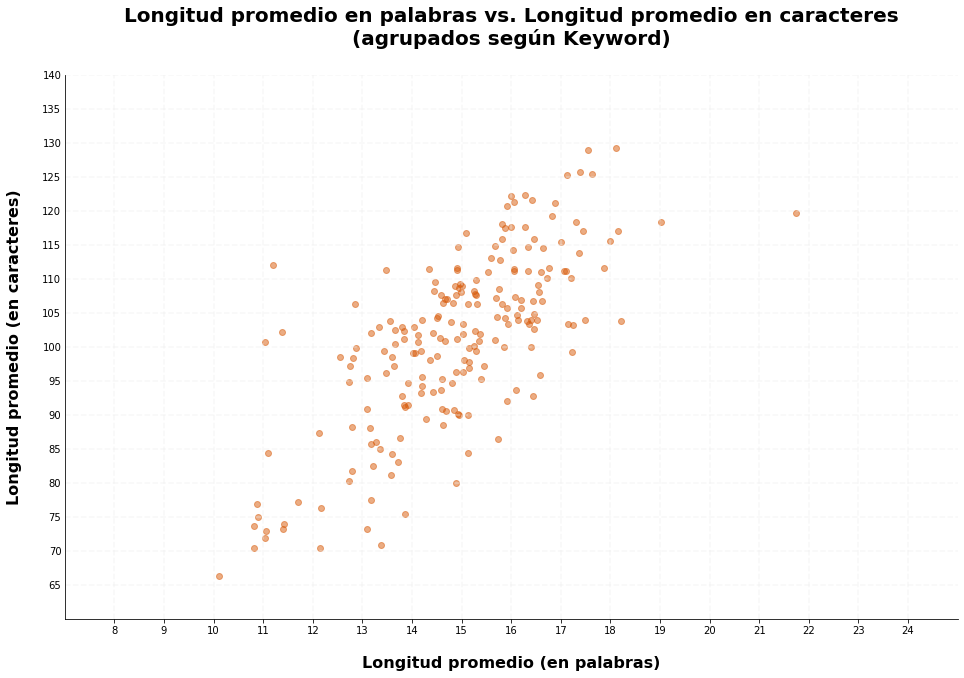
\includegraphics[width=1\textwidth]{graficos/Analisis de Keyword/long_prom_en_palabras_vs_long_prom_en_Caracteres.png}
    \caption{} 
    \end{figure}
    Se observa una relación aproximadamente lineal entre la longitud en caracteres y la longitud en palabras. Esto era de esperar pues al aumentar la cantidad de palabras, debe forzosamente aumentar la cantidad de caracteres. Se nota un punto a la derecha que se encuentra algo distante al resto, este puede ser considerado un \textit{''outlier''} y no es necesario tratarlo con demasiada importancia. Por otro lado se puede deber a que los \textit{Tweets} con dichas \textit{Keywords} si bien en promedio usan más palabras, estas puede que sean cortas explicando así la posición del punto en el gráfico. 
    
    A continuación se procede a analizar la relación que tiene la longitud promedio de los \textit{Tweets} con la veracidad de los mismos agrupados por su \textit{Keyword}. Vale aclarar que a lo largo de esta sección, cuando se habla de veracidad de \textit{Keywords}, se hace referencia al porcentaje de veracidad del grupo de \textit{Tweets} asociado a determinada \textit{Keyword}. Asimismo, la longitud mostrada es la longitud promedio del dicho conjunto de \textit{Tweets}. 
    
    \begin{figure}[H]
    \centering
    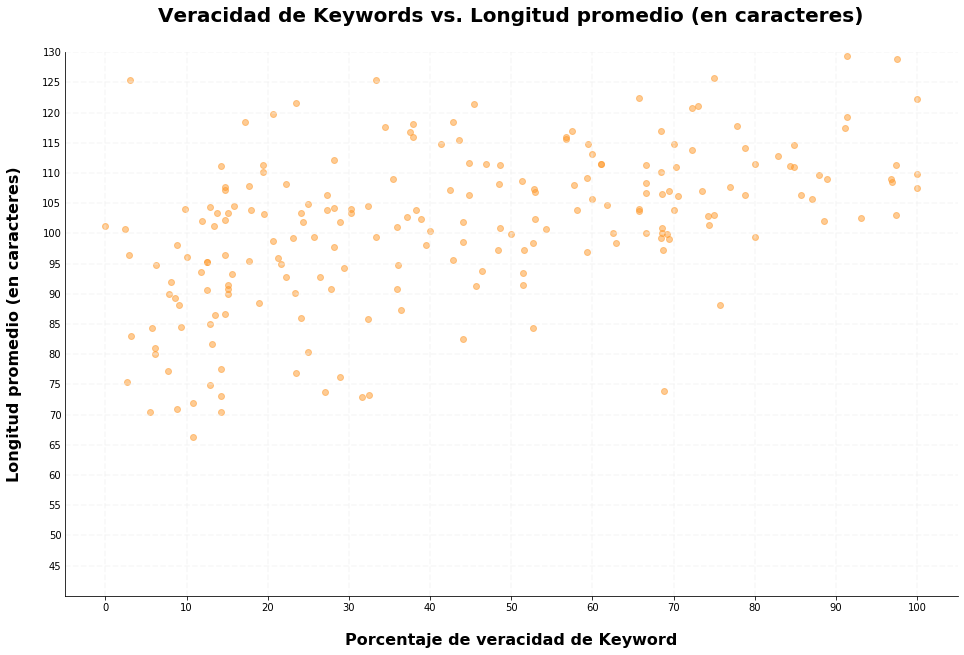
\includegraphics[width=1\textwidth]{graficos/Analisis de Keyword/veracidad_keywords_vs_long_promedio_en_caracteres.png}
    \caption{} 
    \end{figure}
    
    Se puede observar una relación que puede ser considerada como lineal. Lo cual respalda lo ya mencionado en numerosas ocasiones, las \textit{Keywords} asociadas a \textit{Tweets} que en promedio son mas largos, tienden a tener una mayor veracidad.
    
    De igual manera, las \textit{Keywords} que tienen menor veracidad tienden a hacer referencia a \textit{Tweets} de menor longitud
    
    \begin{figure}[H]
    \centering
    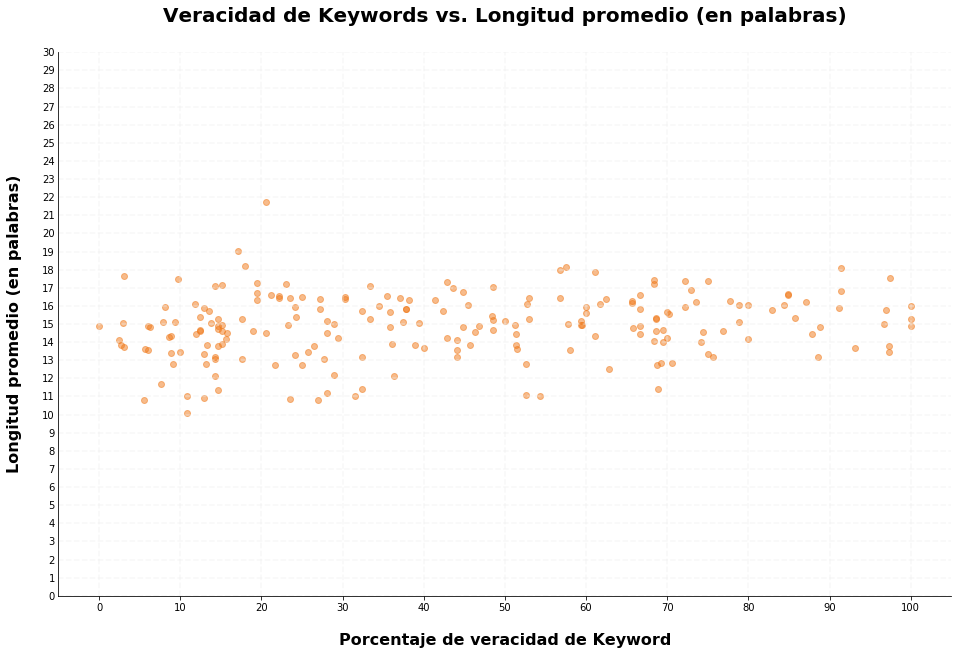
\includegraphics[width=1\textwidth]{graficos/Analisis de Keyword/veracidad_de_keywords_vs_long_promedio_en_palabras.png}
    \caption{} 
    \end{figure}
    
    La distribución de las \textit{Keywords} puede considerarse uniforme respecto de su veracidad. A su vez, todas se encuentran contenidas en una franja considerablemente marcada. De igual manera,puede observarse una concentración ligeramente mayor para los valores de veracidad mas bajos.
    
    \newpage
    
    Los siguientes gráficos resumen la relación que hay tanto entre las \textit{Keywords} mas veraces como las menos veraces con la longitud tanto en caracteres como en palabras de los \textit{Tweets} asociados. Cabe destacar que cuando en los siguientes gráficos se habla de longitud promedio total es en referencia a la longitud promedio del total de los datos mostrados en el gráfico en cuestión y no del total del set.
    
    \begin{figure}[H]
    \centering
    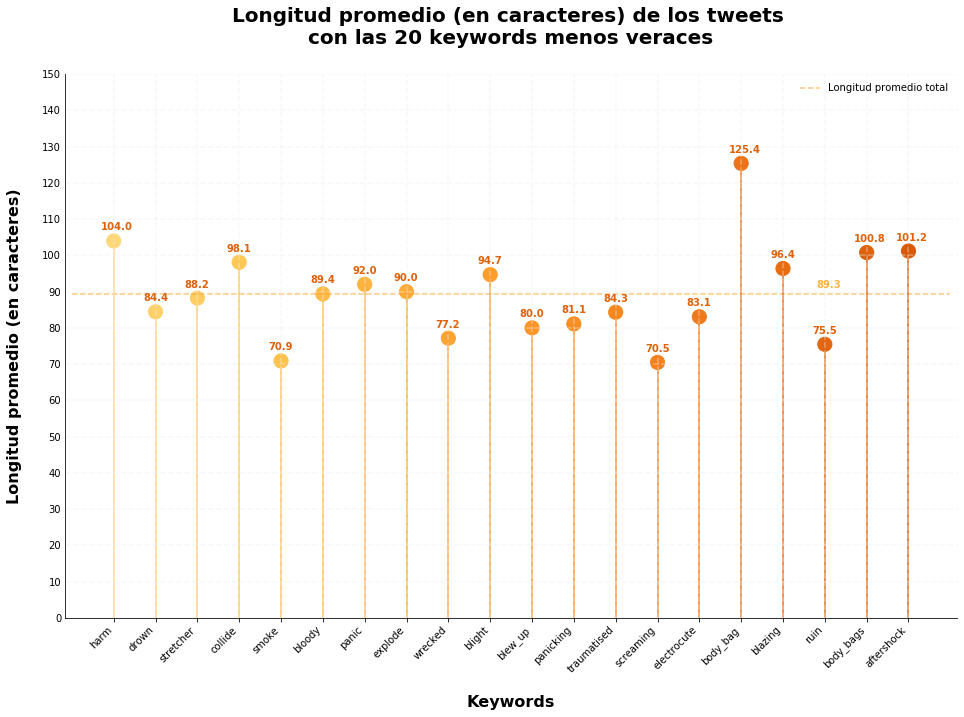
\includegraphics[width=1\textwidth]{graficos/Analisis de Keyword/long_prom_char_keywords_no_veraces.png}
    \caption{} 
    \end{figure}
    
    Se puede observar que la longitud promedio en caracteres de los \textit{Tweets} asociados a las 20 \textit{Keywords} menos veraces esta ligeramente por encima de los 89 caracteres (89,3 caracteres para ser precisos). También se puede ver a simple vista que la \textit{Keyword} \textit{``body\_bag''} que significa ``bolsa para cadáveres'' aunque en ciertos contextos puede interpretarse como un tipo de ``bolso'' o ``cartera'' tiene asociados \textit{Tweets} mas largos con diferencia respecto a las demás, con una longitud promedio de 126 caracteres aproximadamente (126,3 palabras para ser precisos) 
    
    \begin{figure}[H]
    \centering
    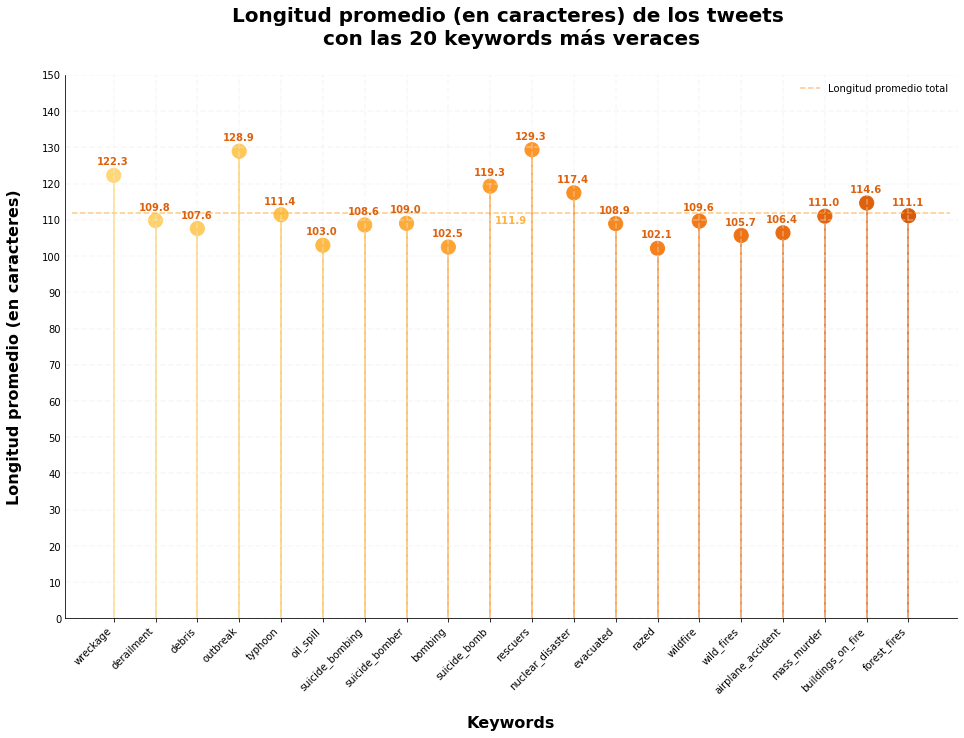
\includegraphics[width=1\textwidth]{graficos/Analisis de Keyword/long_prom_char_keywords_veraces.png}
    \caption{} 
    \end{figure}
    
    Se puede apreciar que todas las longitudes promedio de los \textit{Tweets} asociados a las 20 \textit{Keywords} mas veraces están todas sobre los 100 caracteres y no presentan tanta dispersión como el gráfico anterior. En promedio estas tienen una longitud aproximada de 112 palabras (111,9 palabras para ser mas preciso). También se puede ver a simple vista que los valores de las \textit{\textit{Keywords}} \textit{``rescuers''} que significa ``rescatadores'' y \textit{``outbreak''} que significa ``brote'' destacan sobre el resto por tener una longitud de \textit{Tweets} asociados levemente mayor al resto  
    
    Una observación importante muy fácil de ver es que los \textit{Tweets} que tienen asociadas \textit{Keywords} mas veraces tienden a ser considerablemente mas largos que los que tienen una \textit{Keyword} poco veraz. La diferencia promedio es de \texttt{ 111,9 - 89,3 = 22,6}; Esto puede deberse a que las ``\textit{Keywords} más veraces'', tienen asociados un mayor porcentaje de \textit{Tweets} que efectivamente hacen referencia a desastres/accidentes que las ''\textit{Keywords} menos veraces'' y como se vio anteriormente la longitud en caracteres de los \textit{Tweets} veraces es mayor a la de los falsos.
    
    \newpage
    Análogamente, se procede a estudiar que ocurre con la longitud promedio en palabras de los \textit{Tweets} asociados a las \textit{Keywords} que presentan menor y mayor porcentaje de veracidad.
    
    \begin{figure}[H]
    \centering
    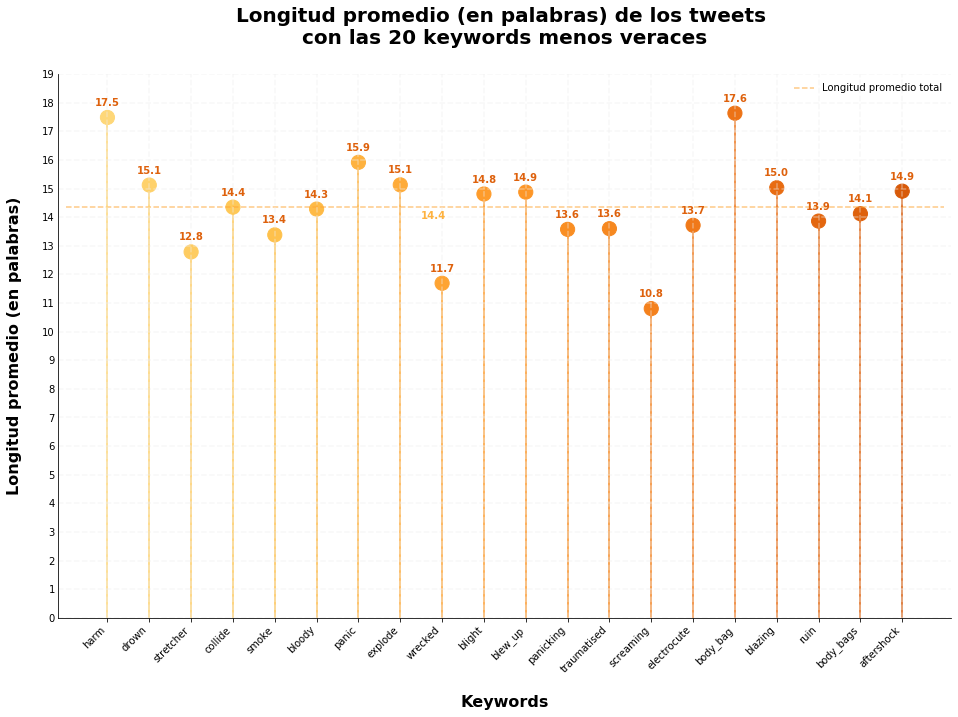
\includegraphics[width=1\textwidth]{graficos/Analisis de Keyword/long_prom_words_keywords_no_veraces.png}
    \caption{} 
    \end{figure}
    
    Se puede apreciar que la longitud promedio es de aproximadamente 14 palabras (14,4 palabras para ser mas preciso). También se puede ver a simple vista que los valores de las \textit{Keywords} ''body\_bag'' y ''harm'' que significa ''daño'' destacan sobre el resto por tener \textit{Tweets} asociados con una longitud en palabras levemente mayor al resto.
     
    
    \begin{figure}[H]
    \centering
    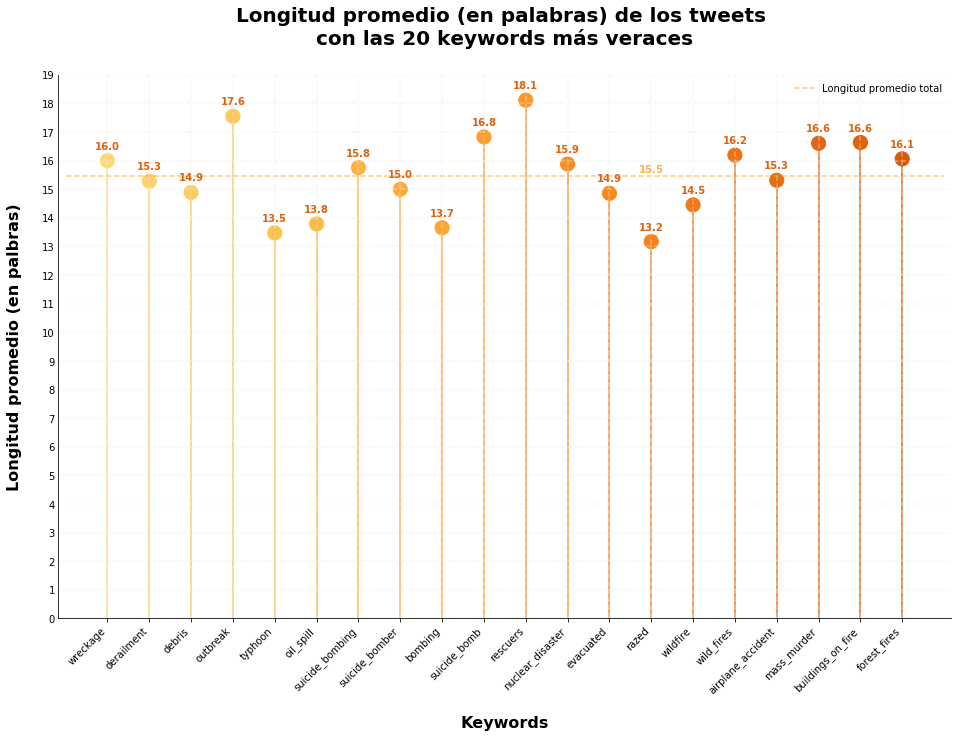
\includegraphics[width=1\textwidth]{graficos/Analisis de Locacion/output_33_1.png}
    \caption{} 
    \end{figure}

    En comparación con la longitud promedio en palabras de los \textit{Tweets} asociados a \textit{Keywords} menos veraces (gráfico anterior), se nota una dispersión de los datos sutilmente menor. También se puede apreciar que la longitud promedio es próxima a 15 palabras (15,5 palabras para ser mas preciso). Con lo cual podemos llegar a la conclusión de que la diferencia en el promedio es de \texttt{ 15,5 - 14,4 = 1,1}.
    
    La diferencia entre la longitud en palabras de los \textit{Tweets} asociados a las \textit{Keywords} mas veraces con respecto a los asociados a las \textit{Keywords} menos veraces es en promedio de 1 palabra (1,1). Esta es una diferencia marcada pero no tan sustancial como en el análisis de la longitud en caracteres, resultado que corrobora lo expuesto anteriormente.
    
    En el siguiente gráfico se puede observar la relación entre la veracidad de las \textit{Keyword} con la cantidad de apariciones de la misma.
    
    \begin{figure}[H]
    \centering
    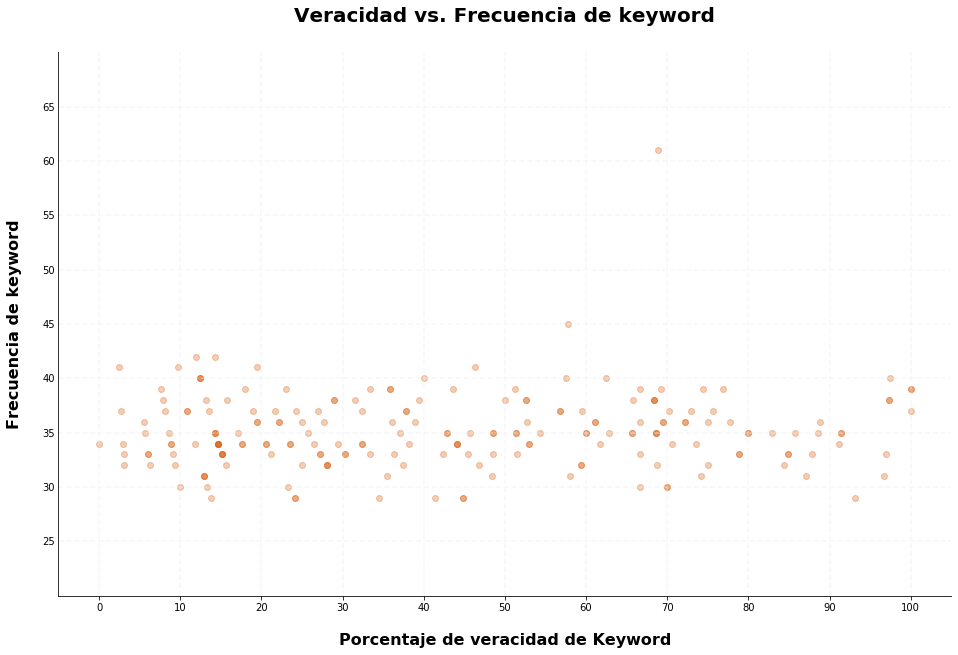
\includegraphics[width=1\textwidth]{graficos/Analisis de Keyword/veracidad_vs_frec_de_keyword.png}
    \caption{} 
    \end{figure}
    
    Como se puede observar la mayoría de las \textit{Keywords} se encuentran en un mismo rango de apariciones que destaca fácilmente como una franja entre los valores de 30 y 40 aproximadamente. Otro punto a destacar es que si bien se observa una mayor concentración en los valores de porcentaje mas bajos, 
    
    \newpage
    \section{Análisis de \textit{Locación}}\label{sec:intro}
    
    En la presente sección se procede a analizar la relación de la locación con otras características de los \textit{Tweets}  
    
    \subsection{Un primer acercamiento a las locaciones}
    
    
    Analizando la cantidad de \textit{Tweets} que tienen una ubicación especificada con respecto a los que no, se llega a la información expresada en el siguiente gráfico. La gran mayoría de \textit{Tweets} tienen una locación especificada (66,7\%).
    
    \begin{figure}[H]
    \centering
    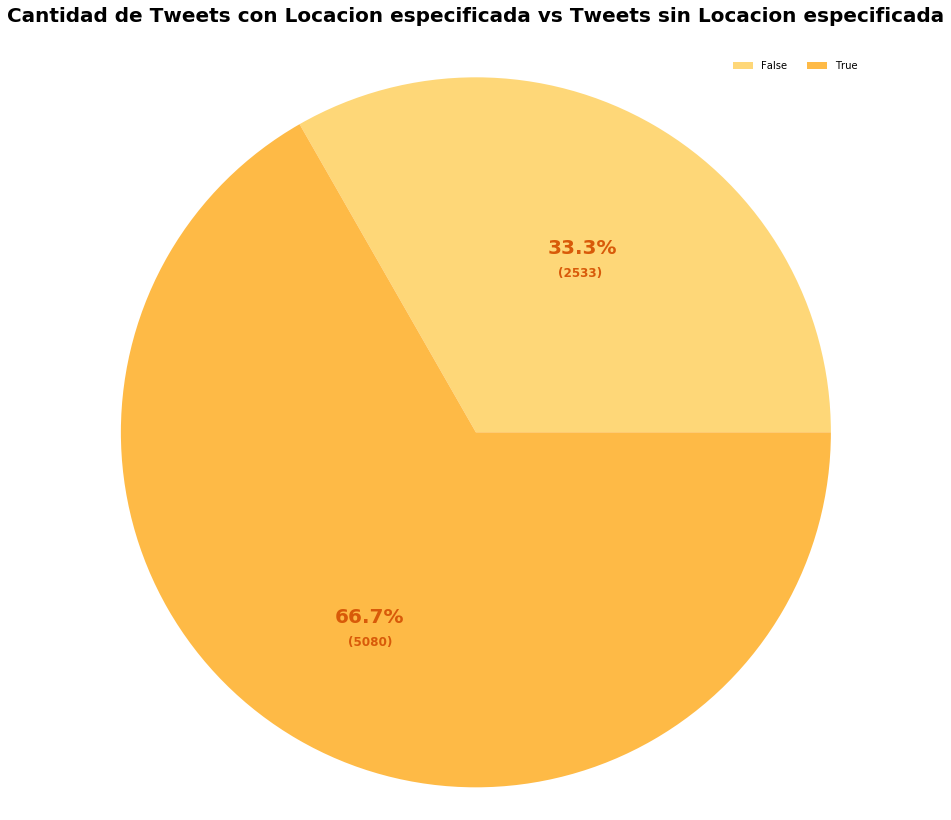
\includegraphics[width=0.9\textwidth]{graficos/Analisis de Locacion/cantidad_de_tweets_con_locacion_especificada_vs_sin_locacion_especificada.png}
    \caption{} 
    \end{figure}
    
    Si contamos la cantidad de apariciones que tiene cada ``\textit{Location}'' sin tener en cuenta aquellos \textit{Tweets} en los que este campo no esta especificado debido a que son considerablemente mas que los \textit{Tweets} cualquier otra locación, con lo cual quedaba sobredimensionado en el gráfico en comparación del resto y por eso se decidió no incluirla.

    \begin{figure}[H]
    \centering
    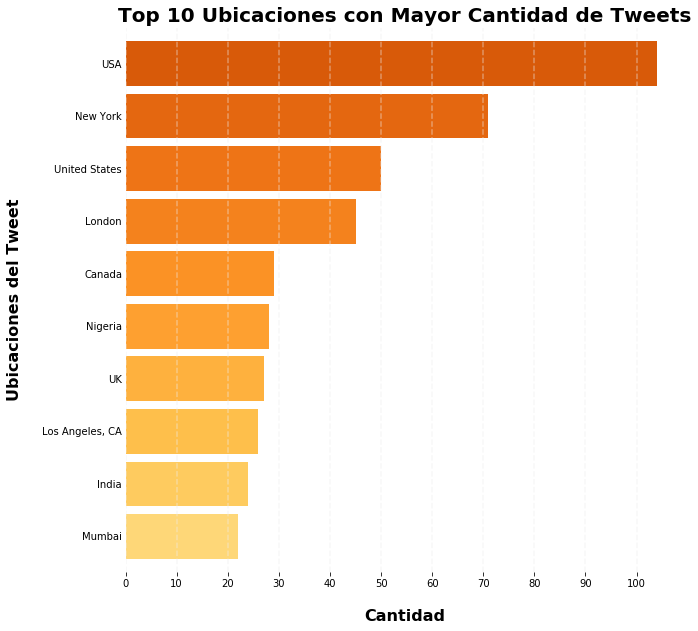
\includegraphics[width=0.9\textwidth]{graficos/Analisis de Locacion/top_10_locaciones_con_mayor_cantidad_de_tweets.png}
    \caption{} 
    \end{figure}
    
    Se puede ver que Estados Unidos es la ubicación con considerablemente mayor cantidad de \textit{Tweets} pues no solo se encuentran dos formas de referirse al mismo en el \textit{Top} (``\textit{USA}'' y ``\textit{United States}'') sino que también se encuentran algunas ciudades de este país. Como se menciono, es importante notar que en el set de datos aparecen sinónimos tanto de ciudades como de países (Ejemplo: ``\textit{NYC}'', ``\textit{New York,}'' y ``\textit{New York City}'' hacen referencia a la misma ciudad pero dentro del set de datos aparecen separadas). Debido a esto, mas adelante procedemos a agrupar estas \textit{``Locations''} sinónimas con el fin de hacer un análisis mas profundo de la información que proveen. 
    
    Se prosigue a analizar cuáles son las locaciones con mayor ratio de \textit{Tweets} relacionados con desastres. El siguiente gráfico muestra las 10 locaciones que presentan mayor porcentaje de veracidad. 
    
    \begin{figure}[H]
    \centering
    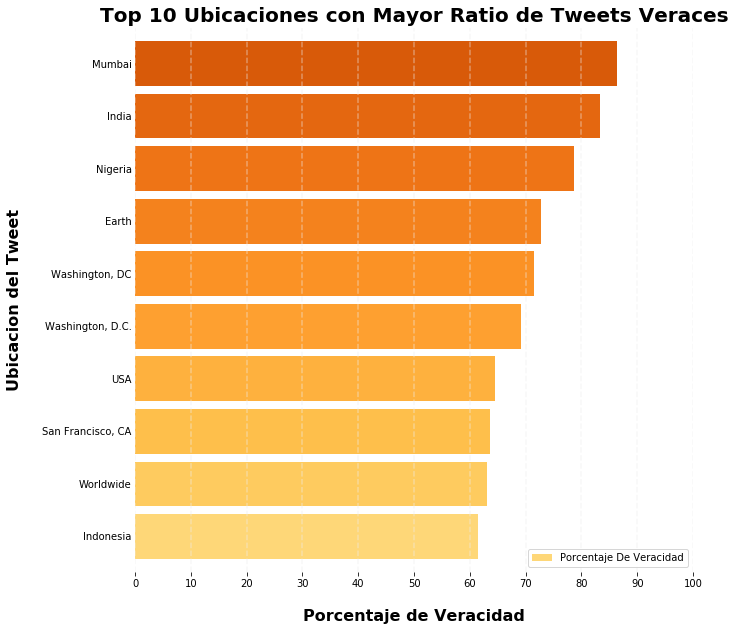
\includegraphics[width=1\textwidth]{graficos/Analisis de Locacion/top_10_locaciones_con_mayor_ratio_de_tweets_veraces.png}
    \caption{} 
    \end{figure}
    
    Se puede apreciar que los \textit{Tweets} de India (Mumbai es una ciudad de India) tienen el mas alto porcentaje de veracidad. 
    
    De manera similar, se analiza las locaciones con mayor ratio de \textit{Tweets} sin relación con desastres (\textit{Tweets} falsos). 
    
    \begin{figure}[H]
    \centering
    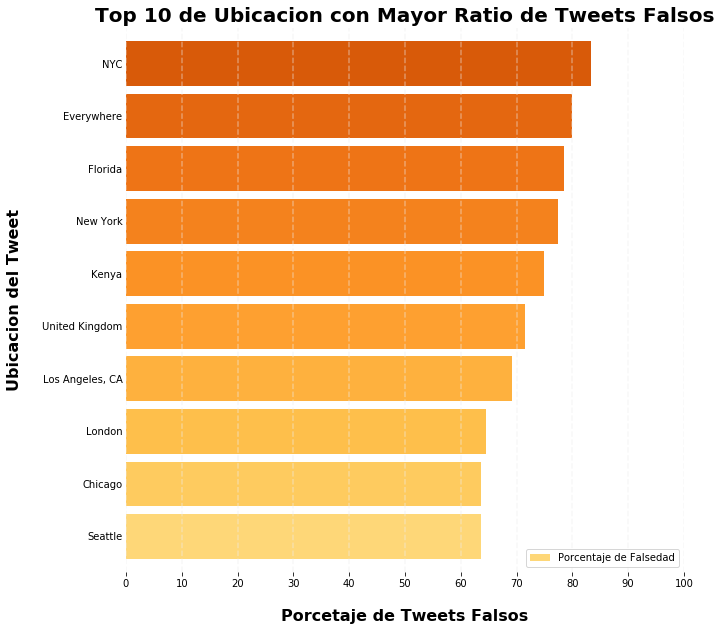
\includegraphics[width=1\textwidth]{graficos/Analisis de Locacion/top_10_locaciones_con_mayor_ratio_de_tweets_falsos.png}
    \caption{}
    \end{figure}
    
    Se puede apreciar una importante presencia de ciudades de Estados Unidos en el \textit{Top} (6 de las 10 entradas). 
    
    \subsection{Análisis por países}
    
    Debido a la variedad de locaciones observadas en estos gráficos y al problema de los sinónimos previamente mencionado, se decidió agrupar los \textit{Tweets} según la ciudad, para posteriormente agruparlos por país de procedencia y, de acuerdo a ello, llevar a cabo los siguientes mapas coropléticos (en inglés, choropleth). Como salvedad se debe mencionar que no fueron tomados en cuenta aquellos \textit{Tweets} en los que no se especifica la ubicación, o aquellos en los que ésta es considerada como inválida.
    
    El criterio de ''válido'' utilizado es que en el campo de ''\textit{Location}'' tiene que estar correctamente escrita la ciudad de procedencia. En base a esto y con ayuda de un csv con información de todas las ciudades del mundo se pueden agrupar los datos de todas las ciudades de cada país para obtener información acerca del país en el que se encuentran.
    
    Como se puede observar, los campos ''\textit{Location}'' que son considerados como válidos según esta convención son una reducida parte del total: 
    
    \begin{figure}[H]
    \raggedleft
    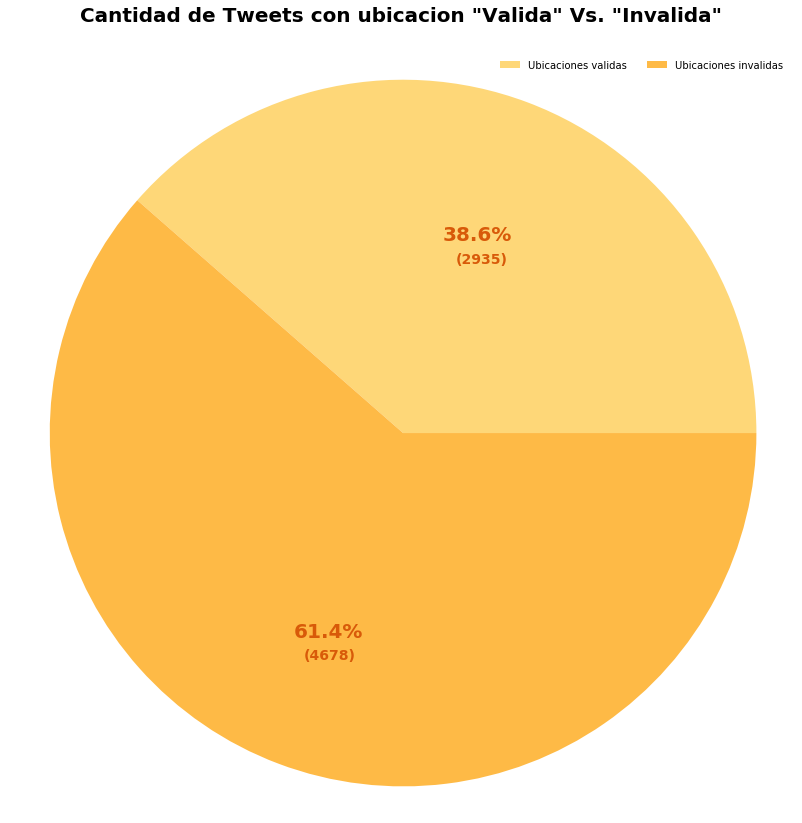
\includegraphics[width=0.9\textwidth]{graficos/Analisis de Locacion/Cantidad_validos_vs_Invalidos.png}
    \caption{}
    \end{figure}
    
    En los siguientes gráficos se puede observar el porcentaje de \textit{Tweets} que efectivamente hace referencia a accidentes verdaderos según el país de procedencia. En este primer gráfico se tuvieron en cuenta los países que tienen por lo menos 1 \textit{Tweet} (aquellos país para los cuales no se encontraron datos aparecen en gris en el gráfico):
    
    \begin{figure}[H]
    \raggedleft
    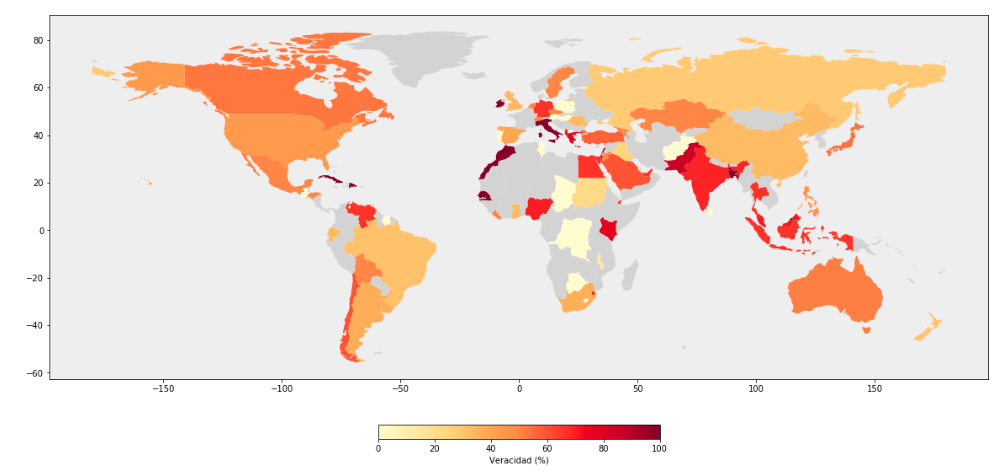
\includegraphics[width=1\textwidth]{graficos/Analisis de Locacion/map1.png}
    \caption{}
    \end{figure}
    
    Se observa que los países del hemisferio norte presentan una tendencia ligeramente mayor a tener un gran porcentaje de \textit{Tweets} referidos tragedias reales, siendo Italia, Marruecos e Irlanda los países que predominan en éste sentido.

    Para este siguiente gráfico se tienen en cuenta solo los países con por lo menos 5 \textit{Tweets}. Esta decisión no es arbitraria si no que dada la cantidad de \textit{Tweets} que tienen la mayoría de países y lo poco distribuidos que estos fueron tomados con respecto a todos los países del mundo (Como se explica posteriormente) se llegó a la conclusión de que esta cantidad puede representar correctamente la veracidad del país a pesar de la limitada muestra.
    
    \begin{figure}[H]
    \raggedleft
    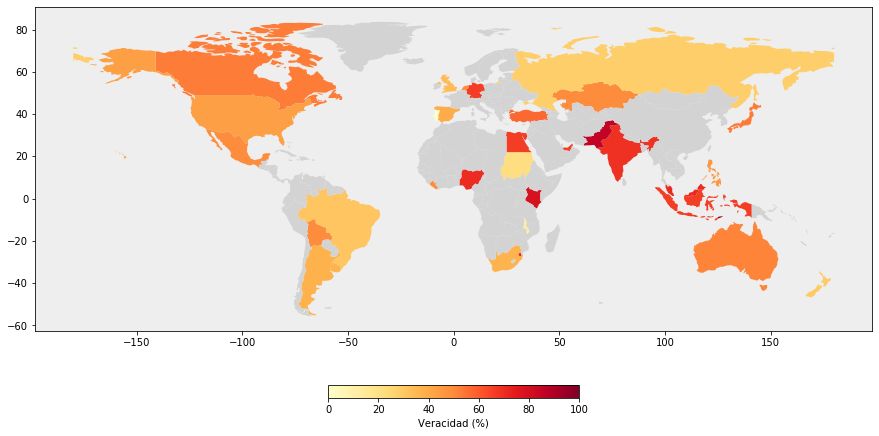
\includegraphics[width=1.1\textwidth]{graficos/Analisis de Locacion/map2.png}
    \caption{}
    \end{figure}  
    
    Como se puede observar, países como Italia, Marruecos e Irlanda, que antes figuraban con una veracidad muy alta, no fueron tenidos en cuenta en este gráfico. Puede interpretarse que los países con poca presencia en el set de datos se ven sobre-representados a ambos extremos de la curva, siendo los que más destacan con mayor y menor veracidad. El análisis de estos datos debe ser tratado con mucho cuidado pues pueden llevar a falsas conclusiones al querer generalizarlos a información de todo el país.
    
    En el siguiente gráfico se exponen los países con mayor cantidad de \textit{Tweets} en escala logarítmica (en base 2):
    
    \begin{figure}[H]
    \centering
    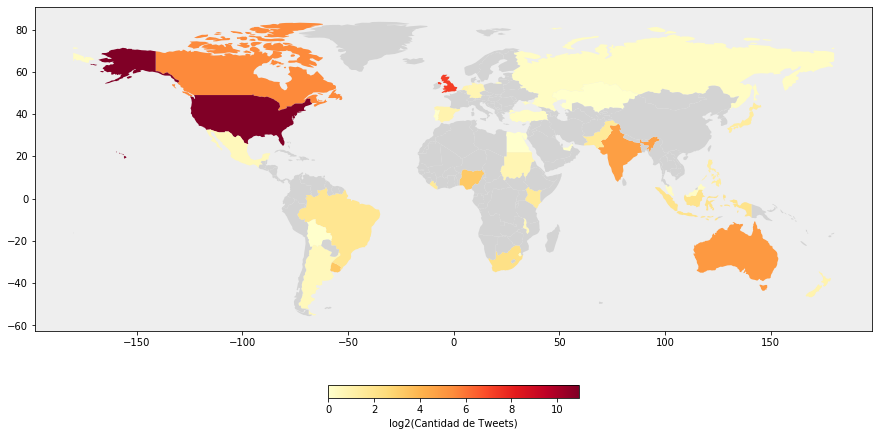
\includegraphics[width=1\textwidth]{graficos/Analisis de Locacion/map_cantidad_tweets.png}
    \caption{}
    \end{figure}
    
    El próximo gráfico muestra la misma información de manera cuantitativa:
    
    \begin{figure}[H]
    \centering
    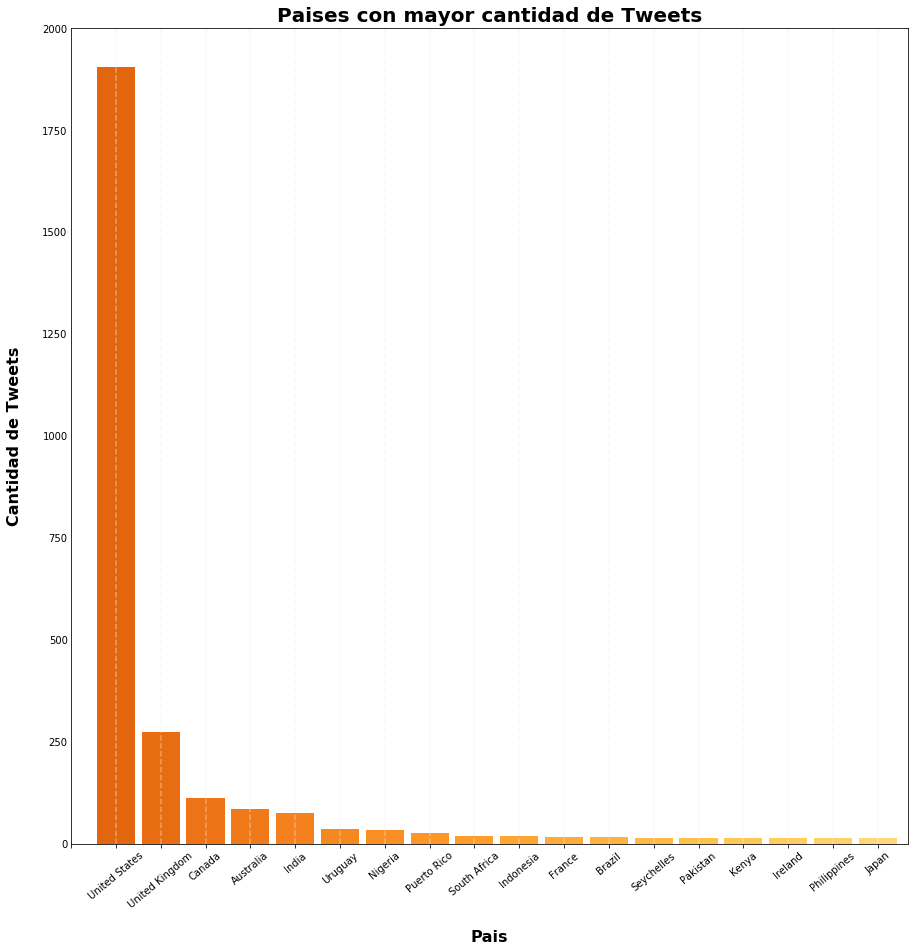
\includegraphics[width=1\textwidth]{graficos/Analisis de Locacion/paises_con_mayor_cantidad_de_tweets.png}
    \caption{}
    \end{figure}
    
    Se expone sin lugar a dudas lo mencionado anteriormente, el país con mas \textit{Tweets} es con diferencia Estados Unidos. También se puede observar que prácticamente la totalidad de los \textit{Tweets} provienen de países de habla inglesa. Esto puede deberse simplemente a  un sesgo al momento de recolectar los datos para el set, prefiriendo, presumiblemente, \textit{Tweets} en ingles y preferentemente provenientes de Estados Unidos.
    
    A continuación, se analiza la veracidad de los \textit{Tweets} por país. Para ello, se filtraron aquellos que tienen más de 10 \textit{Tweets}. Esto es con el fin de que los valores obtenidos sean fieles a la realidad, y no producto de un reducido conjunto de muestras.

    \begin{figure}[H]
    \centering
    \includegraphics[width=1\textwidth]{graficos/Analisis de Locacion/veracidad_promedio_de_los_tweets_por_pais.png}
    \caption{}
    \end{figure}
    
    Como se puede observar entre los países con mayor veracidad promedio, tres de éstos pertenecen al continente africano (Nigeria, Seychelles y Kenya). Además, hay una gran representación de países asiáticos, siendo uno de ellos (Pakistan) el que presenta mayor veracidad promedio de todos los países (Con más de 10 \textit{Tweets}). 
    
    \subsubsection{Análisis de palabras usadas en los cinco países con mayor cantidad de \textit{Tweets}}
    En los siguientes gráficos se exponen las palabras mas usadas en los países con mayor cantidad de \textit{Tweets}, habiendo filtrado pronombres y artículos por razones anteriormente explicadas, cada uno acompañado de una imagen mas llamativa visualmente para representar esto mismo no tan cuantitativamente, en los cuales el tamaño de la palabra representa la cantidad de apariciones que tiene dentro de los \textit{Tweets} que corresponden a ese país.
    
    \begin{figure}[H]
    \centering
    \includegraphics[width=1\textwidth]{graficos/Analisis de Locacion/10_palabras_mas_usadas_usa.png}
    \caption{}
    \end{figure}
    Se puede apreciar que todas las \textit{Keywords} están en ingles, lo cual es esperable debido a ser el idioma nativo del país.

    \begin{figure}[H]
    \centering
    \includegraphics[width=1\textwidth]{graficos/Analisis de Locacion/bandera_usa.png}
    \caption{}
    \end{figure}
    
    \begin{figure}[H]
    \centering
    \includegraphics[width=1\textwidth]{graficos/Analisis de Locacion/10_palabras_mas_usadas_uk.png}
    \caption{}
    \end{figure}
    
    Al igual que con lo ocurrido con Estados Unidos, todas las \textit{Keywords} están en ingles, lengua nativa del país.
    
    \begin{figure}[H]
    \centering
    \includegraphics[width=1\textwidth]{graficos/Analisis de Locacion/bandera_uk.png}
    \caption{}
    \end{figure}

    \begin{figure}[H]
    \centering
    \includegraphics[width=1\textwidth]{graficos/Analisis de Locacion/10_palabras_mas_usadas_canada.png}
    \caption{}
    \end{figure}
    
    
    \begin{figure}[H]
    \centering
    \includegraphics[width=1\textwidth]{graficos/Analisis de Locacion/bandera_canada.png}
    \caption{}    
    \end{figure}
    
    \begin{figure}[H]
    \centering
    \includegraphics[width=1\textwidth]{graficos/Analisis de Locacion/10_palabras_mas_usadas_australia.png}
    \caption{}
    \end{figure}
    
    \begin{figure}[H]
    \centering
    \includegraphics[width=1\textwidth]{graficos/Analisis de Locacion/bandera_australia.png}
    \caption{}
    \end{figure}
    
    \begin{figure}[H]
    \centering
    \includegraphics[width=1\textwidth]{graficos/Analisis de Locacion/10_palabras_mas_usadas_india.png}
    \caption{}
    \end{figure}
    
    Es esperable que una de las \textit{Keywords} mas usadas en India sea ``mh370''. Como ya se comento, esta esta relacionada con el vuelo 370 de Malaysia Airlines. Dentro de este vuelo se encontraban cinco pasajeros de nacionalidad Hindú. Además de haber sido uno de los países que aportaron que se sumo rápidamente a los esfuerzos internacionales de búsqueda del aeronave. Otra \textit{Keyword} que puede estar relacionada con el accidente mencionado es ``Malaysia''.
    
    \begin{figure}[H]
    \centering
    \includegraphics[width=1\textwidth]{graficos/Analisis de Locacion/bandera_india.png}
    \caption{}
    \end{figure}
    
    
    Es destacable que la \textit{Keyword} \textit{``Fire'}' aparece en todas los cinco países analizados. La presencia de esta \textit{Keyword} se muestra principalmente en Canadá y en Australia, ambos países que suelen tener incendios forestales. 
    
    También se observa que de las \textit{Keywords} de los cinco países se encuentran en ingles, lo cual no es extraño en Estados Unidos, Reino Unido, Canadá ni Australia debido a que en dichos países el ingles es la lengua nativa pero en India este no es el caso. Esto se puede deber a cierto sesgo previamente mencionado al momento de la recolección de datos. 
    
    \subsection{Análisis por ciudades}
    
    De igual manera, se calcula la cantidad de \textit{Tweets} por ciudad:
    
    \begin{figure}[H]
    \centering
    \includegraphics[width=1\textwidth]{graficos/Analisis de Locacion/ciudades_con_mayor_cantidad_de_tweets.png}
    \caption{}
    \end{figure}
    
    Este gráfico entra en concordancia una vez mas con lo mencionado anteriormente, ya que prácticamente la totalidad de estas ciudades son de habla inglesa y a su vez la mayoría de ellas se encuentran en Estados Unidos. Esto refuerza la hipótesis de cierto sesgo al momento de la recolección de datos. 
    
    Se prosigue a analizar la veracidad promedio por ciudad:
    
    \begin{figure}[H]
    \centering
    \includegraphics[width=0.95\textwidth]{graficos/Analisis de Locacion/veracidad_promedio_de_los_tweets_por_ciudad.png}
    \caption{}
    \end{figure}
    
    Se puede apreciar que Estados Unidos, no solo tiene ciudades con varios \textit{Tweets} sino que estos también tienen una alta veracidad promedio.
    
    El siguiente gráfico expone la relación entre la veracidad y la cantidad de \textit{Tweets} para cada ciudad (se tomaron las ciudades con mas de 10 \textit{Tweets} por las razones explicadas anteriormente). Al mismo tiempo, el radio de los círculos es proporcional a la raíz cuadrada de la cantidad de habitantes de esa ciudad. Vale aclarar que los colores fueron elegidos arbitrariamente con el fin de ver todos los círculos a pesar de la superposición de los mismos.
    
    \begin{figure}[H]
    \centering
    \includegraphics[width=1\textwidth]{graficos/Analisis de Locacion/veracidad_vs_antidad_de_tweets_por_ciudad.png}
    \caption{}
    \end{figure}
    
    Si bien la cantidad de ciudades con una elevada cantidad de \textit{Tweets} no es suficiente para sacar conclusiones con cierta certeza, se puede observar que la veracidad de las mismas tiende a un 50\%. Esto podría ser un fenómeno que ocurre en todas la ciudades como producto de aumentar el tamaño de la muestra.
    
    Otra observación importante es que las ciudades con mayor cantidad de \textit{Tweets} comparten la característica de tener gran cantidad de habitantes (Círculos grandes) y las ciudades con baja cantidad de \textit{Tweets}, baja cantidad de habitantes (Círculos pequeños).
    
    El siguiente gráfico es similar al anterior; pero en este caso se expone la relación entre la veracidad y la cantidad de habitantes, y en esta ocasión el radio de los círculos es proporcional a la raíz cuadrada de la cantidad de \textit{Tweets} de esa ciudad. Al igual que el anterior gráfico, los colores de los círculos fueron elegidos arbitrariamente para facilitar la visualización:
    
    \begin{figure}[H]
    \centering
    \includegraphics[width=1\textwidth]{graficos/Analisis de Locacion/veracidad_vs_cantidad_de_habitantes_por_ciudad.png}
    \caption{}
    \end{figure}
    
    A diferencia del anterior gráfico, este muestra que mientras más habitantes tiene la ciudad, más tiende a tener alrededor del 50\% de veracidad. También es fácil notar que prácticamente no hay ciudades con veracidad mayor al 80\%.

    \newpage
    \section{Conclusión}\label{sec:intro}

    A lo largo de este análisis exploratorio se buscó estudiar la mayor cantidad posible de características de los \textit{Tweets} y las relaciones existentes entre ellas. Como se mostró en los análisis de resultados posteriores a cada gráfico, se pudieron observar patrones de comportamiento muchas veces considerados ``esperados'' o ``lógicos'', aunque en otras ocasiones no se les pudo asociar un fundamento contundente, demostrando propiedades intrínsecas del set de datos.
    
    Se puede concluir que los \textit{Tweets} que efectivamente hacen referencia a desastres/accidentes reales tienden a tener una longitud en caracteres considerablemente mayor en comparación a los que no. Esta diferencia no es tan apreciable si la medición de longitud se realiza en palabras. 
    
    Una deducción derivada de lo recientemente mencionado es que los Tweets veraces están conformados por palabras de mayor longitud.    
    
    Además, los \textit{Tweets}  que incluyen palabras específicas a una terminología que se pueda asociar con desastres o accidentes tienden a ser veraces en la mayoría de los casos, lo cual es tanto notable como esperable. No sucede lo mismo con los \textit{Tweets} conformados por palabras que pueden ser empleadas en diversos contextos o que simplemente no pertenecen a la terminología que se pueda asociar con desastres.
    
    %Esto justifica por qué las palabras con poca veracidad, puesto a que tienden a ser palabras poco relacionadas con una terminología asociada a desastres y muchas veces, si bien pueden ser utilizadas para describir uno, también pueden ser usadas en otras situaciones. (Uwu)
    
    %De las 30 palabras mas repetidas muchas refieren a desastres, (porque casi la mitad de los Tweets refieren a desastres)
    
    %estas palabras de poca veracidad son la minoría (el lenguaje informal predomina en la red social y nuestro set tiene mas Tweets falsos que verdaderos) HAY MUCHAS CONTRADICCIONES ACA XD
    
    Un comportamiento similar a esto último se puede inferir en los grupos de \textit{Tweets} asociados a la mayoría de las \textit{Keywords}, puesto que poseen un porcentaje de veracidad menor al 50\%. Ésto se debe a que, al igual que lo que ocurre con las palabras, muchas de las \textit{Keywords} pueden asociarse a temáticas pertenecientes tanto al contexto de los desastres/accidentes como a cualquier otro tipo de contexto trivial.
    
    Por otra parte, al referirse a la locación desde donde fueron realizados los \textit{Tweets} también se pueden sacar conclusiones interesantes, aún cuando un tercio de los \textit{Tweets} no tiene una ubicación especificada y sólo un 40\% son consideradas válidas bajo el criterio previamente mencionado.

    Una observación interesante es que el sudeste asiático presenta una tendencia a tener los países con el mayor porcentaje de veracidad de \textit{Tweets}, este resultado muy probablemente esté sujeto a cambios si consideramos una muestra más grande, ya que existe una inclinación a que la veracidad tienda a un 50\% conforme aumentamos el tamaño de la muestra; esto último cuenta tanto para ciudades como para países.
    
    Curiosamente, este mismo fenómeno se manifiesta de manera similar analizando las distintas ciudades según su población; conforme la cantidad de habitantes es mayor, el promedio de veracidad tiende a rondar el 50\%. 
  
    Si bien siempre quedan aspectos sin analizar o que se pasan por alto, se trato contemplar los aspectos que fueron considerados más importantes y representativos de los datos.
    
    
\newpage
    \section{Referencias externas}\label{sec:intro}
    
    \begin{itemize}
        \item Link al repositorio de Github:
            
            \href{https://github.com/hugomlb/TP1-Organizacion-de-Datos}{https://github.com/hugomlb/TP1-Organizacion-de-Datos}
            
    \end{itemize}

\end{document}

